\documentclass[aps, prb, superscriptaddress, longbibliography]{revtex4-2}
%\documentclass[onecolumn,aps,prl,preprint,groupedaddress]{revtex4}
\usepackage{epsfig}
%\usepackage{graphicx}
\usepackage{color}
\usepackage{amsmath}
\usepackage{braket}
%\usepackage{mathabx,graphicx}
%\def\Circlearrowleft{\ensuremath{%
%		\rotatebox[origin=c]{180}{$\circlearrowleft$}}}
%\def\Circlearrowright{\ensuremath{%
%		\rotatebox[origin=c]{180}{$\circlearrowright$}}}
%\def\CircleArrowleft{\ensuremath{%
%		\reflectbox{\rotatebox[origin=c]{180}{$\circlearrowleft$}}}}
%\def\CircleArrowright{\ensuremath{%
%		\reflectbox{\rotatebox[origin=c]{180}{$\circlearrowright$}}}}
\usepackage{amsfonts}
\usepackage{enumitem}
\usepackage{hyperref}
\hypersetup{
	colorlinks = true,
	linkcolor = blue,
	citecolor = blue,
	urlcolor  = blue,
}
%\bibliographystyle{apsrev4-1}
%\usepackage{biblatex}

%\addbibresource{TgrapheneBib.bib}
% You should use BibTeX and apsrev.bst for references
% Choosing a journal automatically selects the correct APS
% BibTeX style file (bst file), so only uncomment the line
% below if necessary.
% \bibliographystyle{apsrev4-1}

\newcommand{\be}{\begin{equation}}
	\newcommand{\ee}{\end{equation}}
\newcommand{\pih}{\frac{2\pi \mathcal{N}}{\hbar}}
\newcommand{\bea}{\begin{eqnarray}}
	\newcommand{\eea}{\end{eqnarray}}
\newcommand{\HH}{{\cal H}}
\newcommand{\RR}{{\cal R}}
\newcommand{\Li}{{\rm Li}}
\newcommand{\p}{\partial}
\newcommand{\s}{\sigma}
\renewcommand{\l}{\lambda}
\newcommand{\la}{\left\langle}
\newcommand{\ra}{\right\rangle}
\newcommand{\lt}{\left|}
\newcommand{\rt}{\right|}
\newcommand{\lb}{\left[}
\newcommand{\rb}{\right]}
\newcommand{\lp}{\left(}
\newcommand{\rp}{\right)}
\newcommand{\sgn}{{\rm sgn\,}}
\newcommand{\tr}{{\rm \, tr\,}}
\renewcommand{\Re}{{\rm \, Re\,}}
\renewcommand{\Im}{{\rm \, Im\,}}
\renewcommand{\vec}[1]{{\bf #1}}
\renewcommand{\phi}{\varphi}
\renewcommand{\epsilon}{\varepsilon}
% \renewcommand{\hat}[1]{{\widehat #1}}
\def\nn{\nonumber\\}
\newcommand{\mpar}[1]{\marginpar{\small \it #1}}
\newcommand{\revision}[1]{\textcolor{blue}{#1}}
\newcommand{\revisionA}[1]{\textcolor{magenta}{#1}}
\newcommand{\revisionB}[1]{\textcolor{red}{#1}}
\newcommand{\addDO}[1]{\textcolor{blue}{#1}}

%very important to save time!
\renewcommand{\cite}[1]{[\onlinecite{#1}]}

\numberwithin{equation}{section}
\begin{document}
	\title{Notes on using graphene as neuromorphic layer of neural network}
	\maketitle
	
	\tableofcontents
	\newpage


\section{Device with perpendicular fall of light with polarization}
\begin{figure}[htbp]
    \centering
    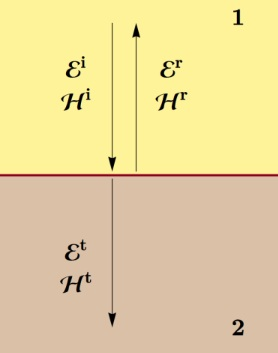
\includegraphics[width=0.2\textwidth]{Figures_for_notes/Kerrs.jpg} % or .pdf, .jpg
    \caption{Illustration for the light scattering on a thin film.}
    \label{fig:my_label}
\end{figure}
\subsection{Floquet reflection and transmission}

Let us model our 2D thin film as a conducting interface on the $x$–$y$ plane, and take light as a plane wave propagating along $z$ direction, i.e., normal incidence. We denote the side with the incident and the reflected light as side 1, and the side with the transmitted light as side 2. We also denote the vectors representing the incident and the reflected electric (magnetic) fields as $\mathbf{E}^i$ ($\mathbf{H}^i$), $\mathbf{E}^r$ ($\mathbf{H}^r$), and that of the transmitted as $\mathbf{E}^t$ ($\mathbf{H}^t$). Notice simple generalization for the multiple harmonics due to different frequencies of each. 

For each Floquet harmonic \(n\) ($n\neq 0$), in vacuum we write
\begin{equation}
\mathbf E_n(\mathbf r,t)=\mathbf E_n e^{i(\mathbf k_n\cdot \mathbf r-\omega_n t)},\qquad\mathbf H_n(\mathbf r,t)=\mathbf H_n e^{i(\mathbf k_n\cdot \mathbf r-\omega_n t)}.
\end{equation}
Then Maxwell equations in source-free vacuum,
\begin{equation}
\nabla\times \mathbf E = -\mu_0 \partial_t \mathbf H,\qquad\nabla\times \mathbf H = \epsilon_0 \partial_t \mathbf E,
\end{equation}
reduce to
\begin{equation}
\mathbf k_n\times \mathbf E_n=\omega_n\mu_0 \mathbf H_n,\qquad\mathbf k_n\times \mathbf H_n=-\omega_n\epsilon_0 \mathbf E_n .
\end{equation}

For the transmitted wave, \(\mathbf k_n=+k_n\hat{\mathbf z}\), hence
\begin{equation}
\mathbf H_n^t=\frac{k_n}{\omega_n\mu_0}\hat{\mathbf z}\times \mathbf E_n^t, \qquad \hat{\mathbf z}\times\begin{pmatrix}E_{n,x}^t\\ E_{n,y}^t\\ 0\end{pmatrix}=\begin{pmatrix}- E_{n,y}^t\\ E_{n,x}^t\\ 0\end{pmatrix},\qquad\frac{k_n}{\omega_n\mu_0}=c\epsilon_0,
\end{equation}
we obtain (for the incident wave calculation is identical with $\mathbf{E}^i_n\sim \delta_{n,1}$)
\begin{equation}
\mathbf H_n^t=c\epsilon_0\begin{pmatrix}- E_{n,y}^t\\ E_{n,x}^t\end{pmatrix},\qquad \mathbf H_n^i=c\epsilon_0\begin{pmatrix}- E_{n,y}^i\\ E_{n,x}^i\end{pmatrix}.
\end{equation}

For the reflected wave, extra $"-"$ sign, \(\mathbf k_n=-k_n\hat{\mathbf z}\), so
\begin{equation}
\mathbf H_n^r=-\frac{k_n}{\omega_n\mu_0}\hat{\mathbf z}\times \mathbf E_n^r=c\epsilon_0\begin{pmatrix}E_{n,y}^r\\ -E_{n,x}^r\end{pmatrix}=-c\epsilon_0\begin{pmatrix}-E_{n,y}^r\\ E_{n,x}^r\end{pmatrix}.
\end{equation}


Continuity of the tangential electric field gives
\begin{equation}\label{continuity}
\boxed{\mathbf E_n^t-\mathbf E_n^i-\mathbf E_n^r=0.}
\end{equation}
The magnetic boundary condition,
\begin{equation}
\hat{\mathbf z}\times(\mathbf H_n^2-\mathbf H_n^1)=\mathbf j_n,
\end{equation}
with \(\mathbf H_n^2=\mathbf H_n^t\) and \(\mathbf H_n^1=\mathbf H_n^i+\mathbf H_n^r\), yields
\begin{equation}
\hat{\mathbf z}\times(\mathbf H_n^t-\mathbf H_n^i-\mathbf H_n^r)=\mathbf j_n.
\end{equation}
Substituting the explicit vacuum relations for \(\mathbf H_n^{t,r,i}\), one finds (very intuitive since $\mathbf{H}^{i/t} = c\varepsilon_0 [\mathbf{z}\times \mathbf{E}^{i/t}], ~\mathbf{H}^{r} = -c\varepsilon_0 [\mathbf{z}\times \mathbf{E}^{r}]$ and $[\mathbf{z}\times[\mathbf{z}\times \mathbf{a}]]=-\mathbf{a}_{\rm in-plane}$)
\begin{equation}
\boxed{\mathbf E_n^t-\mathbf E_n^i+\mathbf E_n^r=-\frac{\mathbf j_n}{c\epsilon_0}.}
\end{equation}
\subsection{Floquet self-consistent transmission}
Importantly, the current appears in the system due to a local electric field, thus according to the Maxwell boundary as in eq.(\ref{continuity}), $\mathbf{j}$ depends on the transmitted component of the light ($z = 0$), 
\begin{equation}
\boxed{\mathbf E_n^t+\frac{\mathbf j_n\left[\{\sum_m\mathbf{E}^t_m e^{-im\Omega t}\}\right]}{2c\epsilon_0}=\mathbf E_n^i,}
\end{equation}
with $|\mathbf{E}^t_m|\sim |\mathbf{E}^i|^m$, allowing the control of convergence.

\subsection{Incident light with in-plane momentum}

We now generalize the previous derivation to oblique incidence. Let the interface be the $x$--$y$ plane at $z=0$, and let the incident light propagate in the $x$--$z$ plane, so that the in-plane momentum is directed along $x$. For each Floquet harmonic $n$, we write
\begin{equation}
\mathbf E_{a,n}^\alpha(\mathbf r,t)=\mathbf E_{a,n}^\alpha\,e^{i(\mathbf k_{a,n}^\alpha\cdot \mathbf r-\omega_n t)},
\qquad
\mathbf H_{a,n}^\alpha(\mathbf r,t)=\mathbf H_{a,n}^\alpha\,e^{i(\mathbf k_{a,n}^\alpha\cdot \mathbf r-\omega_n t)},
\end{equation}
where $\alpha=i,r,t$ labels incident, reflected, and transmitted waves, and $a=1,2$ labels the medium.

For a spatially uniform film, the interface is translationally invariant in the $x$--$y$ plane, and therefore cannot supply in-plane momentum. As a result, the tangential wavevector is conserved for every Floquet harmonic at the interface ($z=0$)
\begin{equation}
    E_{\|}^t-E_{\|}^i=E_{\|}^r \qquad \rightarrow\qquad k_{n,\|}^t=k_{n,\|}^i=k_{n,\|}^r
\end{equation}

\begin{equation}
\mathbf k^\alpha_{a,n,\parallel}=(q,0),
\end{equation}
with the same $q$ for incident, reflected, and transmitted components. The full wavevectors therefore take the form
\begin{equation}
\mathbf k^i_{1,n}=(q,0,k_{z,1,n}),\qquad
\mathbf k^r_{1,n}=(q,0,-k_{z,1,n}),\qquad
\mathbf k^t_{2,n}=(q,0,k_{z,2,n}),
\end{equation}
where
\begin{equation}
k_{z,a,n}=\sqrt{\epsilon_a\mu_a\,\omega_n^2-q^2}.
\end{equation}
Hence each Floquet harmonic has the same in-plane momentum $q$, but its own longitudinal momentum $k_{z,a,n}$ and therefore its own propagation angle
\begin{equation}
\sin\theta_{a,n}=\frac{q}{|\mathbf k^\alpha_{a,n}|}.
\end{equation}
When $q>\sqrt{\epsilon_a\mu_a}\,\omega_n$, the quantity $k_{z,a,n}$ becomes imaginary and the corresponding harmonic is evanescent.

Before imposing Maxwell boundary conditions, it is useful to characterize the allowed electric fields. For a plane wave in a homogeneous medium, transversality requires
\begin{equation}
\mathbf k^\alpha_{a,n}\cdot \mathbf E^\alpha_{a,n}=0.
\end{equation}
Thus for a given wavevector $\mathbf k^\alpha_{a,n}=(q,0,\pm k_{z,a,n})$, the electric field can be decomposed into two transverse polarizations.

Since the plane of incidence is the $x$--$z$ plane, the transverse electric (TE, or $s$) polarization is simply
\begin{equation}
\hat{\mathbf s}=\hat{\mathbf y}.
\end{equation}
The transverse magnetic (TM, or $p$) polarization lies in the plane of incidence and is orthogonal to $\mathbf k^\alpha_{a,n}$. Introducing
\begin{equation}
k_{a,n}=\sqrt{q^2+k_{z,a,n}^2}=\sqrt{\epsilon_a\mu_a}\,\omega_n,
\end{equation}
we define
\begin{equation}
\hat{\mathbf p}^{\,\pm}_{a,n}
=
\hat{\mathbf s}\times \hat{\mathbf k}^{\,\pm}_{a,n}
=
\frac{1}{k_{a,n}}(\pm k_{z,a,n},0,-q),
\end{equation}
where
\begin{equation}
\hat{\mathbf k}^{\,\pm}_{a,n}=\frac{1}{k_{a,n}}(q,0,\pm k_{z,a,n}).
\end{equation}

Therefore, for each harmonic, the most general electric field is
\begin{equation}
\mathbf E^\alpha_{a,n}
=
E^{\alpha,s}_{a,n}\,\hat{\mathbf s}
+
E^{\alpha,p}_{a,n}\,\hat{\mathbf p}^{\,\sigma_\alpha}_{a,n},
\qquad
\sigma_i=\sigma_t=+,\quad \sigma_r=-.
\end{equation}
Explicitly,
\begin{equation}
\mathbf E^\alpha_{a,n}
=
E^{\alpha,s}_{a,n}\begin{pmatrix}0\\1\\0\end{pmatrix}
+
E^{\alpha,p}_{a,n}\frac{1}{k_{a,n}}
\begin{pmatrix}
\sigma_\alpha k_{z,a,n}\\
0\\
-q
\end{pmatrix}.
\end{equation}
For example, the incident field may be written as
\begin{equation}
\mathbf E^i_{1,n}
=
E^{i,s}_{1,n}\begin{pmatrix}0\\1\\0\end{pmatrix}
+
E^{i,p}_{1,n}\frac{1}{k_{1,n}}
\begin{pmatrix}
k_{z,1,n}\\
0\\
-q
\end{pmatrix},
\end{equation}
which automatically satisfies $\mathbf k^i_{1,n}\cdot \mathbf E^i_{1,n}=0$.

The magnetic field follows from Maxwell equations,
\begin{equation}
\mathbf k^\alpha_{a,n}\times \mathbf E^\alpha_{a,n}
=
\omega_n\mu_a\,\mathbf H^\alpha_{a,n}.
\end{equation}
Equivalently,
\begin{equation}
\mathbf H^\alpha_{a,n}
=
\frac{1}{Z_a}\,\hat{\mathbf k}^\alpha_{a,n}\times \mathbf E^\alpha_{a,n},
\qquad
Z_a=\sqrt{\mu_a/\epsilon_a}.
\end{equation}
Using
\begin{equation}
\hat{\mathbf k}\times \hat{\mathbf s}=\hat{\mathbf p},
\qquad
\hat{\mathbf k}\times \hat{\mathbf p}=-\hat{\mathbf s},
\end{equation}
we obtain
\begin{equation}
\mathbf H^\alpha_{a,n}
=
\frac{1}{Z_a}
\left(
E^{\alpha,s}_{a,n}\,\hat{\mathbf p}^{\,\sigma_\alpha}_{a,n}
-
E^{\alpha,p}_{a,n}\,\hat{\mathbf s}
\right).
\end{equation}

Thus the full plane-wave fields can be written as
\begin{equation}
\mathbf E^\alpha_{a,n}(\mathbf r,t)
=
\left(
E^{\alpha,s}_{a,n}\,\hat{\mathbf s}
+
E^{\alpha,p}_{a,n}\,\hat{\mathbf p}^{\,\sigma_\alpha}_{a,n}
\right)
e^{i(qx+\sigma_\alpha k_{z,a,n}z-\omega_n t)},
\end{equation}
\begin{equation}
\mathbf H^\alpha_{a,n}(\mathbf r,t)
=
\frac{1}{Z_a}
\left(
E^{\alpha,s}_{a,n}\,\hat{\mathbf p}^{\,\sigma_\alpha}_{a,n}
-
E^{\alpha,p}_{a,n}\,\hat{\mathbf s}
\right)
e^{i(qx+\sigma_\alpha k_{z,a,n}z-\omega_n t)}.
\end{equation}

At the interface, the relevant driving field for the 2D film is the tangential electric field,
\begin{equation}
\mathbf E_{\parallel}(z=0,t)=\sum_n \mathbf E_{\parallel,n} e^{-i\omega_n t},
\end{equation}
since the sheet current is purely in-plane. The boundary conditions then read, for each harmonic $n$,
\begin{equation}
\boxed{
\mathbf E^{t}_{2,n,\parallel}
-
\mathbf E^{i}_{1,n,\parallel}
-
\mathbf E^{r}_{1,n,\parallel}
=0,
}
\end{equation}
and
\begin{equation}
\boxed{
\hat{\mathbf z}\times
\left(
\mathbf H^{t}_{2,n,\parallel}
-
\mathbf H^{i}_{1,n,\parallel}
-
\mathbf H^{r}_{1,n,\parallel}
\right)
=
\mathbf j_n.
}
\end{equation}
Here $\mathbf j_n$ is the $n$th Floquet harmonic of the sheet current, determined self-consistently by the local tangential electric field at the interface,
\begin{equation}
\mathbf j_n=\mathbf j_n\!\left[\left\{\mathbf E_{\parallel,m}(z=0)\right\}\right].
\end{equation}

This decomposition makes it clear that the oblique-incidence problem is naturally formulated in the TE/TM basis: the TE polarization remains along $\hat{\mathbf y}$, while the TM polarization is obtained by rotating the in-plane polarization so as to remain perpendicular to the corresponding wavevector of each harmonic.
\subsection{Perturbative photo-current}
\addDO{We need to add here references and notation: $f$ are tight-binding hopping functions in Hamiltonian, $\epsilon$ - energies of bands, $A$ - Berry curvature.}


Following the standard multi-band perturbation theory we write that quantum system generally displays the response of the DM as:
\begin{equation}
    \hat\rho^{(1)}_{ab}(t) = -\frac{e}{\hbar}\int d\omega_2E^{j}(\omega_2)e^{-i\omega_2 t}\left(\delta_{ab}\frac{i\partial^jf_a}{\omega_2+i\Gamma}+\frac{f_{ba}A^{j}_{ab}}{\omega_2-\varepsilon_{ab}+i\Gamma}\right),
\end{equation}
\begin{multline}
    \hat{\rho}^{(2)}_{ab}(t)=\frac{e^2}{\hbar^2}\iint d\omega_2d\omega_1E^{j}(\omega_2)E^{i}(\omega_1)e^{-i(\omega_1+\omega_2)t}\Bigg\{
    \delta_{ab}\frac{i\partial^ii\partial^jf_a}{(\omega_1+\omega_2+i\Gamma)(\omega_2+i\Gamma)}+\\+\frac{1}{\omega_1+\omega_2-\varepsilon_{ab}+i\Gamma}i\partial^{i}\frac{A^{j}_{ab}f_{ba}}{\omega_2-\varepsilon_{ab}+i\Gamma}+\\+\frac{A^{i}_{ab}i\partial^jf_{ba}}{(\omega_{2}+i\Gamma)(\omega_1+\omega_2-\varepsilon_{ab}+i\Gamma)}+\frac{1}{\omega_1+\omega_2-\varepsilon_{ab}+i\Gamma}\sum_c\left[\frac{A^i_{ac}A^{j}_{cb}f_{bc}}{\omega_2-\varepsilon_{cb}+i\Gamma}-\frac{A^j_{ac}A^{i}_{cb}f_{ca}}{\omega_2-\varepsilon_{ac}+i\Gamma}\right]\Bigg\}.
\end{multline}
In the Boltzmann limit, we reduce the corresponding currents to ($\omega\ll \Delta$) and $\mathbf{E}_\omega = \sum_l \mathbf{E}^t_{l}\delta(\omega-l\Omega)$:
\begin{equation}
    j^{\gamma, l = 1+2}_{(1)} =-\frac{e^2}{\hbar} \sum_{ab} E^{j, 1}\left(-\delta_{ab}\frac{if_a \partial^j\partial^\gamma \epsilon_a}{\Omega+i\Gamma}+if_{ba}A^{j}_{ab}A^\gamma_{ba}\right)+\frac{e^2}{\hbar} \sum_{ab} E^{j, 2}\left(-\delta_{ab}\frac{if_a \partial^j\partial^\gamma \epsilon_a}{2\Omega+i\Gamma}+if_{ba}A^{j}_{ab}A^\gamma_{ba}\right)
\end{equation}
\begin{equation}
    {j}_{(2),2}^\gamma=\frac{e^3}{\hbar^2}\sum_{ab} E^{j,1}E^{i,1}\Bigg\{
    -\frac{\delta_{ab}f_a \partial^j\partial^i\partial^\gamma \epsilon_a}{(2\Omega+i\Gamma)(\Omega+i\Gamma)}+\frac{iA^\gamma_{ba} A^{i}_{ab}i\partial^jf_{ba}}{\Omega+i\Gamma}\Bigg\}.
\end{equation}
\subsection{Maxwell and microscopic current consistent solution}
By introducing 
\begin{equation}
    (\hat{\sigma}^1_\Omega)_{\gamma j} = -\frac{e^2}{\hbar}\int_\mathbf{k} \sum_{ab}\left(-\delta_{ab}\frac{if_a \partial^j\partial^\gamma \epsilon_a}{\hbar\Omega+i\Gamma}+if_{ba}A^{j}_{ab}A^\gamma_{ba}\right)
\end{equation}
\begin{equation}
    (\hat{\sigma}^2_{\Omega,\Omega})_{\gamma ij} =\frac{e^3}{\hbar}\sum_{ab}\Bigg\{
    -\frac{\delta_{ab}f_a \partial^j\partial^i\partial^\gamma \epsilon_a}{(2\hbar\Omega+i\Gamma)(\hbar\Omega+i\Gamma)}+\frac{iA^\gamma_{ba} A^{i}_{ab}i\partial^jf_{ba}}{\hbar\Omega+i\Gamma}\Bigg\}
\end{equation}
Here we begin to solve the governing equation, to find in the \textbf{linear order}:
\begin{equation}
\boxed{\left(1+\frac{\hat\sigma^1_\Omega}{2c\epsilon_0}\right)\mathbf E_1^t=\mathbf E_1^i,\qquad \mathbf {E}_1^t = \left(1+\frac{\hat\sigma^1_\Omega}{2c\epsilon_0}\right)^{-1}\mathbf {E}_1^i}
\end{equation}
while in the second order:
\begin{equation}
 \boxed{\mathbf{E}_2^{t}=-\frac{1}{2c\varepsilon_0}\left(1+\frac{\hat\sigma^1_{2\Omega}}{2c\epsilon_0}\right)^{-1}\hat{\sigma}^{2}_{\Omega,\Omega}:\mathbf{E}_1^{t}\mathbf{E}_1^{t}}
\end{equation}
where $[\hat{\sigma}^{2}_{2\Omega}:\mathbf{E}_1^{t}\mathbf{E}_1^{t}]_\gamma\equiv E_1^{t,i}E_1^{t,j}(\hat{\sigma}^2_{2\Omega})_{\gamma ij}$. Third order may be introduced later. Schematically, since:
\begin{equation}
    j_3 \sim \sigma^1 E_{3} + \sigma^2 (E_{2}E_1 + E_1 E_2) + \sigma_3 (E_1 E_1E_1) 
\end{equation}
we anticipate:
\begin{equation}
    \boxed{\mathbf{E}_3^{t}=-\frac{1}{2c\varepsilon_0}\left(1+\frac{\hat\sigma^1_{3\Omega}}{2c\epsilon_0}\right)^{-1}\hat{\sigma}^{3}_{\Omega,\Omega,\Omega}:\mathbf{E}_1^{t}\mathbf{E}_1^{t}\mathbf{E}_1^{t}-\frac{1}{2c\varepsilon_0}\left(1+\frac{\hat\sigma^1_{3\Omega}}{2c\epsilon_0}\right)^{-1}\bigg(\hat{\sigma}^{2}_{\Omega,2\Omega}:\mathbf{E}_1^{t}\mathbf{E}_2^{t}+\hat{\sigma}^{2}_{2\Omega,\Omega}:\mathbf{E}_2^{t}\mathbf{E}_1^{t}\bigg)}
\end{equation}
Yet this requires some meaningfull third order conductivity.
\section{Model}
Option 1:
\begin{equation}
H(\mathbf{k})
=
t_x k_x\,\mathbb{1}
+
v k_x \sigma_x
+
v k_y \sigma_y
+
m \sigma_z .
\end{equation}
Unfortunately Drude is UV log divergent. Better:
\begin{equation}
H(\mathbf{k})
=
t_x \sin k_x\,\mathbb{1}
+
v \sin k_x\,\sigma_x
+
v \sin k_y\,\sigma_y
+
\left(m
+
2-\cos k_x-\cos k_y
\right)\sigma_z .
\end{equation}
with $a k_x,a k_y \in [-\pi, \pi]$, $v/vF =1$ ($v_F\sim 10^6$m/s$\sim 2.2$ eV), $m=1/4..1/40$ smaller - stronger BCD. 

\addDO{More restrictions coming from model:} we work in certain frequency range, but that should probably be much lower than van Hove singularity. Then, if we apply many sequential filters, we want $\omega,2\omega,4\omega,\dots < t_{hopping}$.

\newpage

To treat pixels independently, we need to take into account several length scales:
\begin{enumerate}
    \item Optical diffraction coupling — the pixel size should be several wavelengths (on the order of $\mu$m) to suppress diffraction-mediated cross-talk.
    \item Electronic nonlocality inside the material — the standard formulas we use describe transient currents, which should relax on short length and time scales. It may be necessary to assume that each pixel has its own metallic lead to absorb the generated current.
\end{enumerate}

A possible material platform is a time-reversal-symmetric metallic film with broken inversion and rotational symmetries. When driven at sub-gap frequencies, one can exploit the Berry curvature dipole–induced nonlinear Hall effect. The advantage of this mechanism is that it is nonlinear while remaining dissipationless (i.e., it does not absorb optical power).

An additional physical question arises: if the Berry curvature dipole response is dissipationless, where from comes the resource for the current to flow? One possibility is that the current is associated with polarization rotation and acquires angular momentum from the electromagnetic field.

In this case, the DC current component flows out of the pixel into the external circuit.  
If the current is not measured and the circuit impedance is low, then:

\begin{itemize}
    \item It acts as an effective drain,
    \item It prevents charge accumulation within the pixel,
    \item It does not directly influence the AC harmonic components.
\end{itemize}

The only situations in which the DC component may affect the optical response are:

\begin{itemize}
    \item If the DC current modifies the carrier density, (dont think so)
    \item If it produces significant heating, (no)
    \item If it shifts the chemical potential. (don't think so)
\end{itemize}

Therefore, in the weak-drive (perturbative) regime:

\begin{itemize}
    \item The DC current can safely flow into the external circuit,
    \item The harmonic scattering remains unaffected.
\end{itemize}

\newpage
\begin{figure}
    \centering
    
\includegraphics[scale=1.2]{Figures_for_notes/graphene_3d_encoding.pdf}
    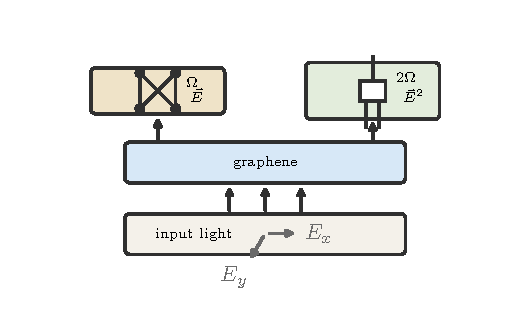
\includegraphics[scale=1.0]{Figures_for_notes/graphene_as_KAN_part_small.pdf}
    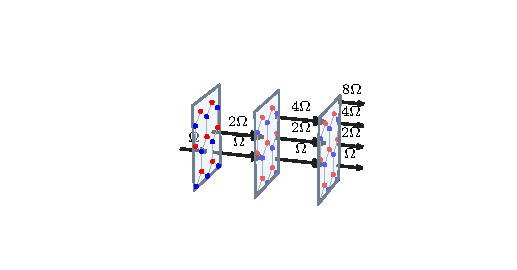
\includegraphics[scale=1.3]{Figures_for_notes/graphene_3d_multipassing.pdf}
    \caption{Possible pixels input through graphene devices?}
    \label{fig:example-device-pixels}
\end{figure}

\subsection{Estimations of available  filters and frequency ranges}
Let us understand the operations that we have in terms of ML. Linear optical transmission is simple - it is a dense linear layer of input - output. E.g, in the simplest scenario it is 
\begin{align}
    \vec{E}_{out}^{t}=\boldsymbol{W}\vec{E}_{in}^{i};\quad \{\vec{E}_{out,1}^{t},\vec{E}_{out,2}^{t},\dots\}=\text{diag}\{\boldsymbol{W},\boldsymbol{W},\dots\}\{\vec{E}_{in,1}^{i},\vec{E}_{in,2}^{i},\dots\}.
\end{align}
However, if we have many input fields coming as different pixels, that is a block-diagonal transformation.

Next, we have a fun tensor-type second order. That brings a new transformation:
\begin{align}
    E_{out,r}^{t, (2)}=\tilde{W}_{l,j,r} E_{in,l}^{i} E_{in,j}^{i}
\end{align}
This looks like a tensor network element, or a tensor processing unit. At the same time, this format would be still local on the field. We could also check the compositions of the field, but firstly we suppose that image really comes as separate in space EM field fronts. This is similar to the quadratic layer of KAN networks. However, this has one more upgrade - since this is a vector format, we get also products of inputs encoded in x- and y-components of E field.

\addDO{So, what do we need to resolve?} 

- Showing that quadratic filter is good - is not the target of this work. Target is to show that graphene could be used in this way!

- Then, what does ``this way'' mean?

- Graphene instead of reflector - cool idea, might improve quality of passed images! For this we need to compare with those filters in terms of quality of output. And then show simple ML benchmark with filter, but that would be well-known, up to particular selection of parameters.

- More novel idea: show that in this way graphene does a layer of KAN. What do we need for that? Seems not much - basically, estimate some sizes, etc, and show how to extract data from $E_x E_y$ products. 

- Tunable? That could be helpful for neuromorphic computing. Encoding in phases? That is also possible

\begin{figure}
    \centering
    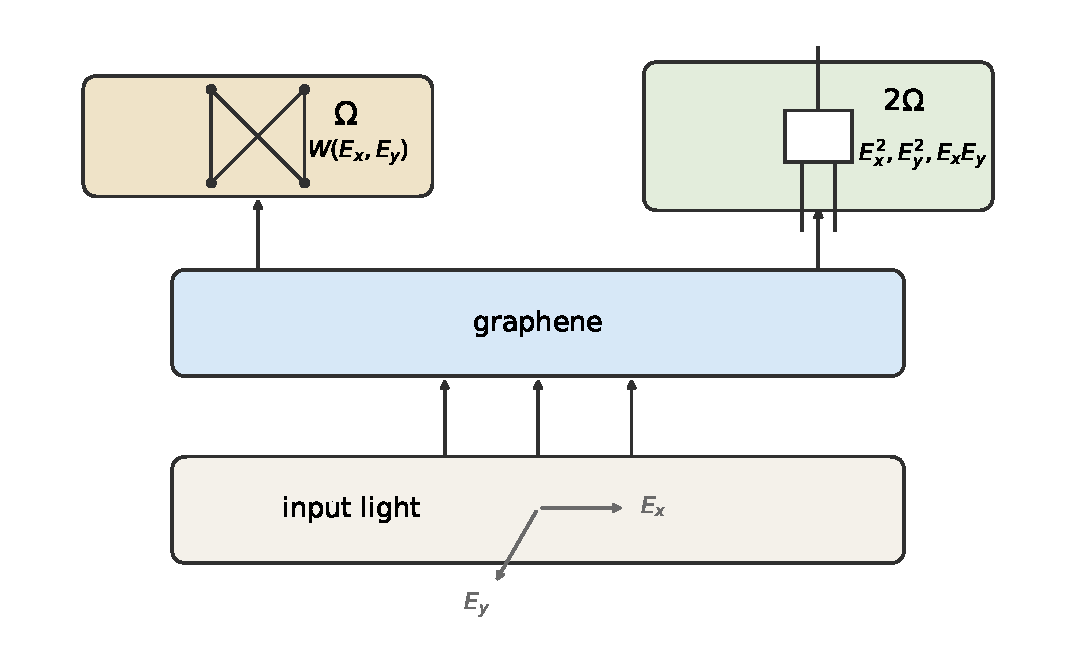
\includegraphics[width=0.75\linewidth]{graphene_as_KAN_part.pdf}
    \caption{Graphene as KAN 2.0 schematics}
    \label{fig:graphene-KAN}
\end{figure}

\subsection{Multi-layer filtering device}
\addDO{Important: investigate frequencies - ladders of them compared to band}
\begin{figure}
    \centering
    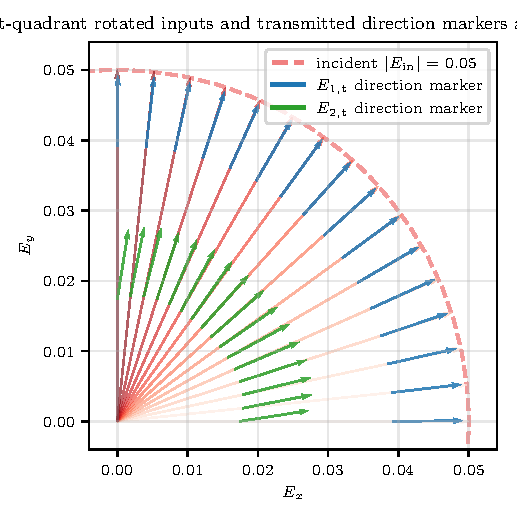
\includegraphics[scale=1.0]{Figures_for_notes/quiver_plot_transmitted_directions_single_surface_test.pdf}
    \caption{Quiver plot indicating directions of transmitted E-field, $(|E_x|,|E_y|)$.}
    \label{fig:quiver-single-surface-test}
\end{figure}

\begin{figure}
    \centering
    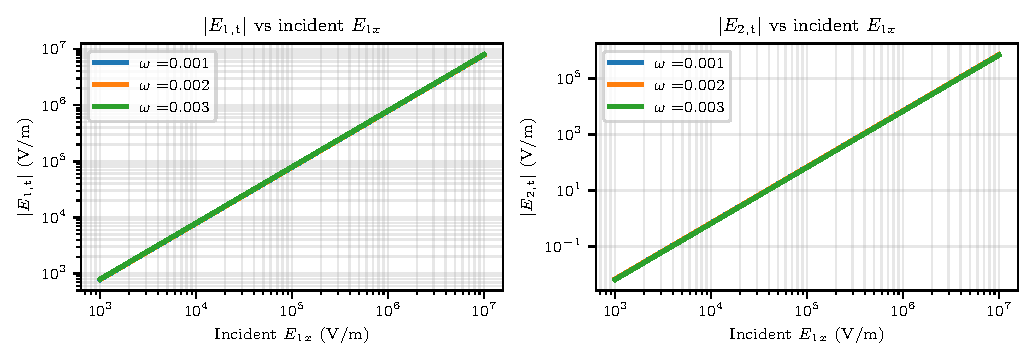
\includegraphics[scale=1.0]{Figures_for_notes/transmitted_harmonics_amplitudes_single_surface.pdf}
    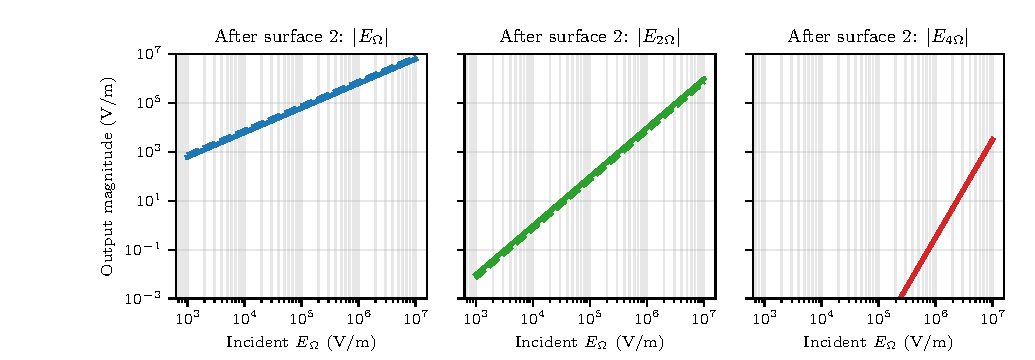
\includegraphics[scale=1.0]{Figures_for_notes/transmission_amplitude_plots_2_surf_device_test.pdf}
    \caption{Two transmitted plots: by 1 (upper) surface and by 2 (lower) surfaces.}
    \label{fig:1-and-2-surface-amplitude-transmission}
\end{figure}


\subsection{Dependence of filters on parameters of the system}
In this section we need to provide a number of plots of conductivities versus system parameters. Suppose frequency is fixed, then what could we tune for neuromorphic scenario?


\subsection{DO: estimation of decoherence / spread of bandwidth?}


\section{Notes on papers about linear optics computing}
Let's discuss mathematical tricks used in each of papers cited below. The main problem that they try to tackle is the same - optical devices typically perform linear transformation only $y_{out}=W x_{in}$. That is of course cool for linear algebra, but more interesting is to generate cheap nonlinearity. 

First paper to consider is {\bf Yildirim et. al.} \cite{Yildirim2024}. They use only linear devices, but do the following trick (non
linear processing with only linear optics): they put ``data of image'' not in the input light, but in the liquid-crystal spatial light modulator. That results in the following algebra:
\begin{align}
E_{\text {out }}=H T_{\mathrm{L} n}(\mathbf{x}) \ldots H T_{\mathrm{L} 2}(\mathbf{x}) H T_{\mathrm{L} 1}(\mathbf{x}) E_{\text {i}} \,\, \text{$E_i$ is not a data!}
\end{align}
So, the data is processed as this:
\begin{align}
\begin{aligned}
o_i= & \sum_{j=1}^K h_{i j}\left(s_j^{(N)} x_j+b_j^{(N)}\right)\left(\ldots \sum_{j=1}^K h_{i j}\left(s_j^{(2)} x_j+b_j^{(2)}\right)\left(\sum_{j=1}^K h_{i j}\left(s_j^{(1)} x_j+b_j^{(1)}\right)\right) \ldots\right)=\sum_{m=0}^N \alpha_{i, m}(\mathbf{s}, \mathbf{b}) \mathbf{x}^m
\end{aligned}
\end{align}
Or as Supplement explains, the result is composed from input, propagations and modulations. And we put data into modulation layer rather than in input:
\begin{align}
&o=\text{propagation}\,\text{modulation}\dots  \text{input}, \\
&\text{one step:}\,\,
\left[\begin{array}{l}
o_1 \\
o_2
\end{array}\right]=\left[\begin{array}{ll}
h_{11} & h_{12} \\
h_{21} & h_{22}
\end{array}\right]\left[\begin{array}{ll}
t_1 & 0 \\
0 & t_2
\end{array}\right]\left[\begin{array}{l}
i_1 \\
i_2
\end{array}\right],\\
&\left[\begin{array}{l}
o_1 \\
o_2
\end{array}\right]=\left[\begin{array}{ll}
h_{11} & h_{12} \\
h_{21} & h_{22}
\end{array}\right]\left[\begin{array}{ll}
t_1 & 0 \\
0 & t_2
\end{array}\right]\left[\begin{array}{l}
h_{11} t_1 i_1+h_{12} t_2 i_2 \\
h_{21} t_1 i_1+h_{22} t_2 i_2
\end{array}\right]=\left[\begin{array}{l}
h_{11}^2 t_1^2 i_1+h_{11} h_{12} t_2 t_1 i_2+h_{12} h_{21} t_1 t_2 i_1+h_{12} h_{22} t_2^2 i_2 \\
h_{21} h_{11} t_1^2 i_1+h_{21} h_{12} t_2 t_1 i_2+h_{22} h_{21} t_1 t_2 i_1+h_{22}^2 t_2^2 i_2
\end{array}\right].
\end{align}
Last result is already nonlinear in transformation - modulation, so information tranformed by a polynomial filter. 

Next thing - how do they compare qualities of performance or energy consumption? Their benchmarks are:

- test dataset accuracies for fashion and digit MNIST datasets, and Imagenette. Received up to 88\% on MNIST, which is kinda low, but not bad for physical system.

- Scaling of performance with number of trainable parameters. Not the best metric, as for MNIST etc it was shown that architecture is more important (like dropout layers, matchnorm, etc).

Second paper - {\bf Wang et.al.}  \cite{Wang2024NatureCommSc}, about large-scale photonic computing. 


Third paper - {\bf Xia, Gigan group} \cite{Xia2024}, about implementing nonlinearities. Idea is the same - hide data not in ``input light'', but in the scattering potential. Performance:

- 80\% of fashion MNIST. 

- some hand-vaiwing about power consumption, and that reflections don't introduce extra power consumptions compared to other active nonlinearities.

\subsection{Note on structure of networks used}
Actually, networks were very simple. In other words, \cite{Yildirim2024} passed data through several optical layers and then used one-layer classifier on a very condensed images. Example description (from chatGPT):
\begin{itemize}
    \item \textbf{For Fashion-MNIST / Digit-MNIST:}
    \begin{itemize}
        \item Input image: $28 \times 28$
        \item Linear upsampling to $75 \times 75$
        \item Mapping onto the SLM using $4 \times 4$ superpixels inside a $300 \times 300$ illuminated area
        \item Optical layer 1: phase mask $\phi_1 = x s_{L1} + b_{L1}$, followed by propagation
        \item Optical layer 2: phase mask $\phi_2 = x s_{L2} + b_{L2}$, followed by propagation
        \item Optical layer 3: phase mask $\phi_3 = x s_{L3} + b_{L3}$, followed by propagation
        \item Optical layer 4: phase mask $\phi_4 = x s_{L4} + b_{L4}$, followed by propagation
        \item Camera detection of output intensity $|E_{\mathrm{out}}|^2$
        \item Average pooling to a $4 \times 4$ feature map for Fashion-MNIST
        \item Flatten
        \item Digital linear classifier with 10 outputs
        \item Softmax / cross-entropy during training
    \end{itemize}

    \item \textbf{For Imagenette:}
    \begin{itemize}
        \item Input image: $320 \times 320$
        \item Linear downsampling to $300 \times 300$
        \item Optical layer 1: phase mask $\phi_1 = x s_{L1} + b_{L1}$, followed by propagation
        \item Optical layer 2: phase mask $\phi_2 = x s_{L2} + b_{L2}$, followed by propagation
        \item Optical layer 3: phase mask $\phi_3 = x s_{L3} + b_{L3}$, followed by propagation
        \item Optical layer 4: phase mask $\phi_4 = x s_{L4} + b_{L4}$, followed by propagation
        \item Camera detection of output intensity $|E_{\mathrm{out}}|^2$
        \item Average pooling to an $8 \times 8$ feature map
        \item Flatten
        \item Digital linear classifier with 10 outputs
        \item Softmax / cross-entropy during training
    \end{itemize}
\end{itemize}


    \subsection{A short summary of typical neural network layers}
    
    \begin{table}[htbp]
\centering
\caption{Standard neural network layers, their mathematical operations, trainability, and usual training method.}
\label{tab:nn_layers}
\begin{tabular}{|l|p{7.2cm}|c|p{3.2cm}|}
\hline
\textbf{Layer} & \textbf{Mathematical operation} & $\begin{array}{c}
\text{Trainable}\\
\text{parameters?}\end{array}$ & \textbf{Usually trained with} \\
\hline
Input layer & $y = x$ & No & Not trained \\
\hline
Dense / Fully connected (Linear) & $y = Wx + b$ & Yes & Gradient descent / backprop \\
\hline
Convolutional & $y_{i,j,k} = \sum_{u,v,c} W_{u,v,c,k} x_{i+u,j+v,c} + b_k$ & Yes & Gradient descent / backprop \\
\hline
Transposed convolution & $\begin{array}{c}
\text{Learned upsampling via}\\
\text{linear convolution transpose} \end{array}$ & Yes & Gradient descent / backprop \\
\hline
Embedding & $y = E[i]$ for token/index $i$ & Yes & Gradient descent / backprop \\
\hline
Bias layer / affine shift & $y = x + b$ & Yes & Gradient descent \\
\hline
Batch normalization & $y = \gamma \dfrac{x-\mu}{\sqrt{\sigma^2+\epsilon}} + \beta$ & Yes & Gradient descent for $\gamma,\beta$ \\
\hline
Layer normalization & $y = \gamma \dfrac{x-\mu}{\sqrt{\sigma^2+\epsilon}} + \beta$ & Yes & Gradient descent \\
\hline
Instance / Group normalization & $\begin{array}{c}
\text{Normalization over selected}\\
\text{axes with affine rescaling}\end{array}$ & Yes & Gradient descent \\
\hline
ReLU & $y = \max(0,x)$ & No & Not trained \\
\hline
Leaky ReLU / PReLU & $y = \max(\alpha x, x)$ & Sometimes & Gradient descent if $\alpha$ is trainable \\
\hline
Sigmoid & $y = \sigma(x) = \dfrac{1}{1+e^{-x}}$ & No & Not trained \\
\hline
Tanh & $y = \tanh(x)$ & No & Not trained \\
\hline
Softmax & $y_i = \dfrac{e^{x_i}}{\sum_j e^{x_j}}$ & No & Not trained directly \\
\hline
Pooling (max / average) & $\begin{array}{c}
\text{Max}: y = \max(x_{\text{window}});\\ 
\text{Avg}: y = \dfrac{1}{n}\sum x_{\text{window}}\end{array}$ & No & Not trained \\
\hline
Global average pooling & $y_c = \dfrac{1}{HW}\sum_{i,j} x_{i,j,c}$ & No & Not trained \\
\hline
Dropout & $y = m \odot x$, with $m_i \sim \mathrm{Bernoulli}(1-p)$ & No & Not trained \\
\hline
Residual / skip connection & $y = F(x) + x$ & Only inside $F$ & Gradient descent \\
\hline
Attention (scaled dot-product) & $\mathrm{Attn}(Q,K,V)=\mathrm{softmax}\!\left(\dfrac{QK^\top}{\sqrt{d_k}}\right)V$ & Yes & Gradient descent / backprop \\
\hline
Multi-head attention & $\begin{array}{c}
\text{Parallel attention heads,}\\ \text{concatenate, then project}\end{array}$ & Yes & Gradient descent \\
\hline
Recurrent layer (RNN) & $h_t=\phi(W_x x_t + W_h h_{t-1}+b)$ & Yes & Gradient descent through time \\
\hline
LSTM & $\begin{array}{c}
\text{Gate-based recurrence with}\\ \text{learned affine transforms}\end{array}$ & Yes & Gradient descent / BPTT \\
\hline
GRU & $\begin{array}{c}
\text{Gated recurrence with}\\
\text{learned affine transforms}\end{array}$ & Yes & Gradient descent / BPTT \\
\hline
Output linear layer & $y = Wx+b$ & Yes & Gradient descent \\
\hline
Output activation (sigmoid / softmax) & Maps logits to probabilities & No & Not trained directly \\
\hline
\end{tabular}
\end{table}

The Table \ref{tab:nn_layers} summarized many of usual NN layers. Still, some more are missing or should be explained. In particular:
\begin{enumerate}
    \item $1\times 1$ convolution - suppose input is a picture of $28\times 28\text (pixels)\times 3\,\text(RGB colors)$. Then, such convolution is $1\times 1\times 3$, so convolution in color space.

    \item Depthwise convolutional layer (DwConv) - one separate filter for each channel. In example of images above - 3 filters, each applied to $28\times28$ image in color.

    \item Graph neural networks: layer transformation is
    \begin{align}
        H^{(\ell+1)}=\sigma\left(\tilde{D}^{-1 / 2} \tilde{A} \tilde{D}^{-1 / 2} H^{(\ell)} W^{(\ell)}\right)
    \end{align}
    $H^{(\ell)}$ : current node features; 
$W^{(\ell)}$ : learnable weight matrix;
$\tilde{A}=A+I$, $A$ - adjacency matrix : passes messages between neighbors; 
$\tilde{D}^{-1 / 2} \tilde{A} \tilde{D}^{-1 / 2}$ : normalized aggregation; 
$\sigma$ : activation, for example ReLU.
    Idea of entire network - each node becomes updated with weight, then information is gathered over neighbors, and then nonlinearity.\\

\item MLP: unstructured vectors. 
GNN: graphs and relations. 
VQC: quantum circuit model, usually for small-feature classical inputs or quantum-native data.
\end{enumerate}



\begin{table}[htbp]
\centering
\caption{Typical Kolmogorov--Arnold network (KAN) layers and their operations.}
\label{tab:kan_layers}
\begin{tabular}{|l|p{7.5cm}|c|p{3.0cm}|}
\hline
\textbf{Layer} & \textbf{Mathematical operation} & $\begin{array}{c}
\text{Trainable}\\
\text{parameters?}\end{array}$ & \textbf{Usually trained with} \\
\hline
Input layer & Passes input vector forward, $y=x$ & No & Not trained \\
\hline
KAN hidden layer & 
For each output component,
\[
y_j = \sum_{i=1}^{n} \phi_{ij}(x_i),
\]
where each $\phi_{ij}$ is a learnable univariate function (often spline-based) & Yes & Gradient descent / backprop \\
\hline
Spline / basis-function edge activation & 
A learnable 1D function expanded in basis functions, e.g.
\[
\phi_{ij}(x)=\sum_{m} c_{ijm} B_m(x)
\]
with basis functions $B_m$ and coefficients $c_{ijm}$ & Yes & Gradient descent \\
\hline
KAN output layer & 
Same additive functional form as hidden KAN layer,
\[
y_j = \sum_{i=1}^{n} \phi_{ij}(x_i)
\]
mapping hidden features to outputs & Yes & Gradient descent / backprop \\
\hline
Optional residual / linear branch & 
Combined linear and nonlinear mapping, e.g.
\[
y = Wx + \sum_i \phi_i(x_i)
\]
or residual addition $y = F(x)+x$ & Sometimes & Gradient descent \\
\hline
\end{tabular}
\end{table}


\section{Important references to keep in mind / cite}
\cite{Taglietti2026arxiv} - Learning Nonlinear Heterogeneity in Physical Kolmogorov-Arnold Networks, nice idea on implementing that in physical platform.

\cite{Wang2024NatureCommSc} - Large-scale photonic computing with nonlinear disordered media

\cite{Xia2024} - Nonlinear optical encoding enabled by recurrent linear scattering

\cite{Yildirim2024} - Nonlinear processing with linear optics

\cite{Hafez2018} - Extremely efficient terahertz high-harmonic generation in graphene by hot Dirac fermions

\cite{Kanega2024} - High-harmonic generation in graphene under the application of a DC electric current:
From perturbative to nonperturbative regime

\cite{Yoshikawa2017} - High-harmonic generation in graphene enhanced by elliptically polarized light excitation

\cite{liu2024kan20kolmogorovarnoldnetworks} -  KAN 2.0: Kolmogorov-Arnold Networks Meet Science

\cite{Zhou2019NatureNanotech} - Optoelectronic resistive random access memory for neuromorphic vision sensors

\cite{Tong2024NatureComm} - Programmable nonlinear optical neuromorphic computing with bare {2D} material {M}o{S}2

\cite{Zhang2024NatureComm} - High performance artificial visual perception and recognition with a plasmon-enhanced {2D} material neural network

\cite{Wang2020SciAdv} - Gate-tunable van der Waals heterostructure for reconfigurable neural network vision sensor

\cite{Mennel2020Nature} - Ultrafast machine vision with {2D} material neural network image sensors

\cite{Choi2025npjUnconvComp} - Advanced {AI} computing enabled by {2D} material-based neuromorphic devices

\cite{Xie2025} - 2{D} Materials for Emerging Neuromorphic Vision: From Devices to In‐Sensor Computing

\cite{Zhao2024BrainX} - Research progress and applications of optoelectronic synaptic devices based on {2D} materials

\cite{Chen2023KeAi} - {2D}-materials-based optoelectronic synapses for neuromorphic applications

\cite{Zhou2019review} - {2D} Materials Based Optoelectronic Memory: Convergence of Electronic Memory and Optical Sensor

\cite{Taglietti2026ArxivLearningNonlinearHeterogeneity} - Learning Nonlinear Heterogeneity in Physical Kolmogorov-Arnold Networks

Important notes:  – how to train 2 nonlinearities to make one KAN in parallel. We could show the same if we have frequency dependence or something like that or two graphene parts controlled / strained differently. Good benchmarking, testing on experiment and also good ideas on how to make more multi-variate functions. Out-of-chip optimization as well. And here we have analogue of some quadratic splines.

\cite{Zhou2025HundredLayer} - Hundred-layer photonic deep learning

\cite{Chen2025Photonics} - Incoherent Optical Neural Networks for Passive and Delay-Free Inference in Natural Light

\cite{Wang2025Light} - Optical next generation reservoir computing. 

Important notes: Idea – optically generate linear and nonlinear parts to make time series next-generation reservoir computing predictions. For nonlinearity they use phase encoding, SLM. So in exponent. This represents the same idea as before in Yildirim and Ginan papers. Reservoir computing – interesting idea itself, especially with this approach. Good for our benchmark purposes.




\section{Short meeting notes}
{\bf 21/02/2026}

1. We discussed about how people in linear optical neuromorphic computed encoded input - through Born scattering, which generated nonlinearity in potential.

2. Also around that time we discussed the switch from conducting device to optical device. Nice to compete with optics people!

..\\
{\bf 08/03/2026}

1.	We want to discard interband transitions;

2.	Nonlinear Hall part;

3.	Frequencies estimation - at some moment we need to estimate which frequency ranges for 1st, 2nd, harmonics are good

4.	Justin at some moment mentioned the idea, where device + trained ML output reader basically composes a good detector. But here it is better - good filter with predictable / testable properties, and then ML that works with that.

5.	Possible feedback loop to tune filter dynamically during ML training;

6.	The plan about noisy input / output signals - how to reasonably simulate the 

7.	Question about which material to use to leverage most of possible operations. E.g., topologival insulator with broken inversion, and probably with selected axis. What is that? Or do we want to we want to make a table of materials as filters?

8. We want to make a plan for numerical simulation: encoding dataset with some noisy input; and then decode and train neural network with our filter and demonstrate efficiency. Btw, here might be also useful to make a table of building blocks in most of standard neural networks.

...\\
{\bf 15/03/2026}

1. We planned to test image + filtered nonlinear data for benchmarking as NN input (done for mnist and fashion mnist).

2. Table of materials as filters is a promising thing!

3. Discussion with chatGPT: good benchmarks could be done on "Mnist, Fashion-MNIST
Breast Cancer Wisconsin
Wine Quality" datasets. Still, one needs to decide on punchline and also on specific / variable neural network architectures plus neuromorphic-motivated benchmarks. E.g., if we do this layer almost for free - what does it give? How to not enhance the cost of computing / classifying layer - summing up $X$+$X^2$?

\newpage\section{Derivation of the DM}

We use the Fourier transform convention
\begin{equation}
    f(\omega)=\int dt\, f(t)e^{i\omega t},
    \qquad
    f(t)=\int \frac{d\omega}{2\pi}\, e^{-i\omega t}f(\omega).
\end{equation}

We will also use the identity
\begin{equation}\label{rcomm}
\boxed{
[ r^\alpha , O ]_{nm}
=
i\partial^{\alpha}_{\mathbf k} O_{nm}
+
[A^\alpha , O]_{nm}
}
\end{equation}
where $A^\alpha_{nm}(\mathbf k)$ is the Berry connection.

A multiband theory applicable to both metals and insulators can be constructed by introducing relaxation phenomenologically in the spirit of the relaxation–time approximation. The density matrix $\hat\rho$ obeys the non–Hermitian Liouville equation
\begin{equation}\label{eq01}
i\hbar\frac{d}{dt}\hat\rho(t)
-
[\hat H,\hat\rho(t)]
=
-i\frac{\hat\rho(t)-\hat\rho_0}{\tau},
\qquad
\hat H=\hat H_0+\hat H_E .
\end{equation}

Here $\tau$ is the relaxation time, $\hat\rho_0$ is the equilibrium density matrix, $\hat H_0$ is the unperturbed tight–binding Hamiltonian, and $\hat H_E$ describes the coupling to the electric field in the length gauge.

We assume that the density matrix deviates only weakly from equilibrium and write
\begin{equation}
\hat\rho=\hat\rho^e+\hat\sigma,
\qquad
[\hat H_0,\hat\rho^e]=0 .
\end{equation}

In the band basis
\begin{equation}
\rho^e_{nm}
=
\delta_{nm}f(\epsilon_n),
\qquad
(H_0)_{nm}
=
\epsilon_n(\mathbf k)\delta_{nm},
\end{equation}
where $n,m$ are band indices, $\epsilon_n(\mathbf k)$ is the band dispersion, and
$f(\epsilon_n)\equiv f_n$ is the Fermi–Dirac distribution.

For convenience we introduce the shorthand
\begin{equation}
f_{nm}=f_n-f_m,
\qquad
\epsilon_{nm}=\epsilon_n-\epsilon_m .
\end{equation}

Substituting $\hat\rho=\hat\rho^e+\hat\sigma$ into Eq.~(\ref{eq01}) gives
\begin{equation}
i\hbar\partial_t\hat\sigma
-
[\hat H_0,\hat\sigma]
-
[\hat H_E,\hat\rho^e]
-
[\hat H_E,\hat\sigma]
=
-i\frac{\hat\sigma}{\tau}.
\end{equation}

To simplify the equation we move to the interaction picture with respect to $\hat H_0$,
\begin{equation}
\hat\sigma(t)
=
U(t,t_0)\,\hat\Sigma(t)\,U^\dagger(t,t_0),
\qquad
U(t,t_0)=e^{-i(t-t_0)\hat H_0/\hbar}.
\end{equation}



In this representation the evolution equation becomes
\begin{equation}
i\hbar\partial_t\hat\Sigma
=
e^{i(t-t_0)\hat H_0/\hbar}
\left(
[\hat H_E(t),\hat\rho^e]
+
[\hat H_E(t),\hat\sigma(t)]
\right)
e^{-i(t-t_0)\hat H_0/\hbar}
-i\frac{\hat\Sigma}{\tau}.
\end{equation}

Equivalently, introducing the interaction-picture perturbation
\begin{equation}
\hat H_E^I(t)=U^\dagger(t,t_0)\hat H_E(t)U(t,t_0),
\end{equation}
and using $[\hat H_0,\hat\rho^e]=0$, so that $\hat\rho^e$ is unchanged in the interaction picture, one may write
\begin{equation}
i\hbar\partial_t\hat\Sigma
=
[\hat H_E^I(t),\hat\rho^e]
+
[\hat H_E^I(t),\hat\Sigma]
-i\frac{\hat\Sigma}{\tau}.
\end{equation}
we rewrite it as
\begin{equation}
\partial_t\hat\Sigma+\frac{\hat\Sigma}{\tau}
=
\frac{1}{i\hbar}[\hat H_E^I(t),\hat\rho^e]
+
\frac{1}{i\hbar}[\hat H_E^I(t),\hat\Sigma].
\end{equation}

Multiplying by the integrating factor $e^{t/\tau}$ gives
\begin{equation}
\partial_t\!\left(e^{t/\tau}\hat\Sigma(t)\right)
=
e^{t/\tau}
\left[
\frac{1}{i\hbar}[\hat H_E^I(t),\hat\rho^e]
+
\frac{1}{i\hbar}[\hat H_E^I(t),\hat\Sigma(t)]
\right].
\end{equation}
Integrating from $t_0$ to $t$, we obtain the exact integral equation
\begin{equation}
\hat\Sigma(t)
=
e^{-(t-t_0)/\tau}\hat\Sigma(t_0)
+
\frac{1}{i\hbar}\int_{t_0}^t dt'\,
e^{-(t-t')/\tau}
\left(
[\hat H_E^I(t'),\hat\rho^e]
+
[\hat H_E^I(t'),\hat\Sigma(t')]
\right).
\end{equation}

Next we expand the density matrix in powers of the electric field,
\begin{equation}
\hat\Sigma(t)=\sum_{n=0}^{\infty}\hat\Sigma^{(n)}(t),
\qquad
\hat\Sigma^{(n)}\sim E^n.
\end{equation}

Assuming vanishing initial perturbation, the first-order correction is
\begin{equation}
\boxed{
\hat\Sigma^{(1)}(t)
=
\frac{1}{i\hbar}\int_{t_0}^t dt'\,
e^{-(t-t')/\tau}
[e^{i(t'-t_0)\hat H_0/\hbar}\hat H_E(t')e^{-i(t'-t_0)\hat H_0/\hbar},\hat\rho^e]
}
\end{equation}
and the higher-order terms satisfy the recursion relation
\begin{equation}
\boxed{
\hat\Sigma^{(n+1)}(t)
=
\frac{1}{i\hbar}\int_{t_0}^t dt'\,
e^{-(t-t')/\tau}
[\hat H_E^I(t'),\hat\Sigma^{(n)}(t')],
\qquad n\ge 1.
}
\end{equation}
with $\hat \rho^{(n)} =e^{i(t-t_0)\hat H_0/\hbar}\hat \Sigma^{(n)}e^{-i(t-t_0)\hat H_0/\hbar}$


\subsubsection{Results}
\begin{equation}
    \hat\rho^{(1)}_{ab}(t) = -\frac{e}{\hbar}\int d\omega_2E^{j}(\omega_2)e^{-i\omega_2 t}\left(\delta_{ab}\frac{i\partial^jf_a}{\omega_2+i\Gamma}+\frac{f_{ba}A^{j}_{ab}}{\omega_2-\varepsilon_{ab}+i\Gamma}\right)
\end{equation}
\begin{multline}
    \hat{\rho}^{(2)}_{ab}(t)=\frac{e^2}{\hbar^2}\iint d\omega_2d\omega_1E^{j}(\omega_2)E^{i}(\omega_1)e^{-i(\omega_1+\omega_2)t}\Bigg\{
    \delta_{ab}\frac{i\partial^ii\partial^jf_a}{(\omega_1+\omega_2+i\Gamma)(\omega_2+i\Gamma)}+\\+\frac{1}{\omega_1+\omega_2-\varepsilon_{ab}+i\Gamma}i\partial^{i}\frac{A^{j}_{ab}f_{ba}}{\omega_2-\varepsilon_{ab}+i\Gamma}+\\+\frac{A^{i}_{ab}i\partial^jf_{ba}}{(\omega_{2}+i\Gamma)(\omega_1+\omega_2-\varepsilon_{ab}+i\Gamma)}+\frac{1}{\omega_1+\omega_2-\varepsilon_{ab}+i\Gamma}\sum_c\left[\frac{A^i_{ac}A^{j}_{cb}f_{bc}}{\omega_2-\varepsilon_{cb}+i\Gamma}-\frac{A^j_{ac}A^{i}_{cb}f_{ca}}{\omega_2-\varepsilon_{ac}+i\Gamma}\right]\Bigg\}
\end{multline}
\begin{equation}
    \rho^{(2)}_{nm}(t)=\frac{e^2}{\hbar ^2}\iint \frac{d\omega_2d\omega_1}{(2\pi)^2}E^{\alpha}(\omega_2)E^{\beta}(\omega_1)e^{-i(\omega_1+\omega_2)t+2\eta t} \chi_{D,nm}^{\alpha\beta}(\omega_1,\omega_2),
\end{equation}
thus
\begin{equation}
    [\hat\rho_{3}(t)]_{nm} = \frac{e^3}{\hbar ^3}\iiint \frac{d\omega_3d\omega_2d\omega_1}{(2\pi)^3}E^\gamma(\omega_3)E^{\alpha}(\omega_2)E^{\beta}(\omega_1)e^{-it(\omega_1+\omega_2+\omega_3)+3\eta t)} \frac{[{r}^\gamma,\chi^{\alpha\beta}(\omega_1,\omega_2)]_{nm}}{\omega_1+\omega_2+\omega_3-\omega_{nm}+3i\eta},
\end{equation}
consider the current

\begin{equation}
    j^{3} = \frac{e^3}{\hbar ^3}\sum_{nm}v^\gamma_{mn}\iiint \frac{d\omega_3d\omega_2d\omega_1}{(2\pi)^3}E^\gamma(\omega_3)E^{\alpha}(\omega_2)E^{\beta}(\omega_1)e^{-it(\omega_1+\omega_2+\omega_3)+3\eta t)} \frac{[{r}^\gamma,\chi^{\alpha\beta}(\omega_1,\omega_2)]_{nm}}{\omega_1+\omega_2+\omega_3-\omega_{nm}+3i\eta},
\end{equation}

\newpage
	\section{Graphene assisted learning (Desn't work so far)}
    \begin{figure}[t]
        \centering
        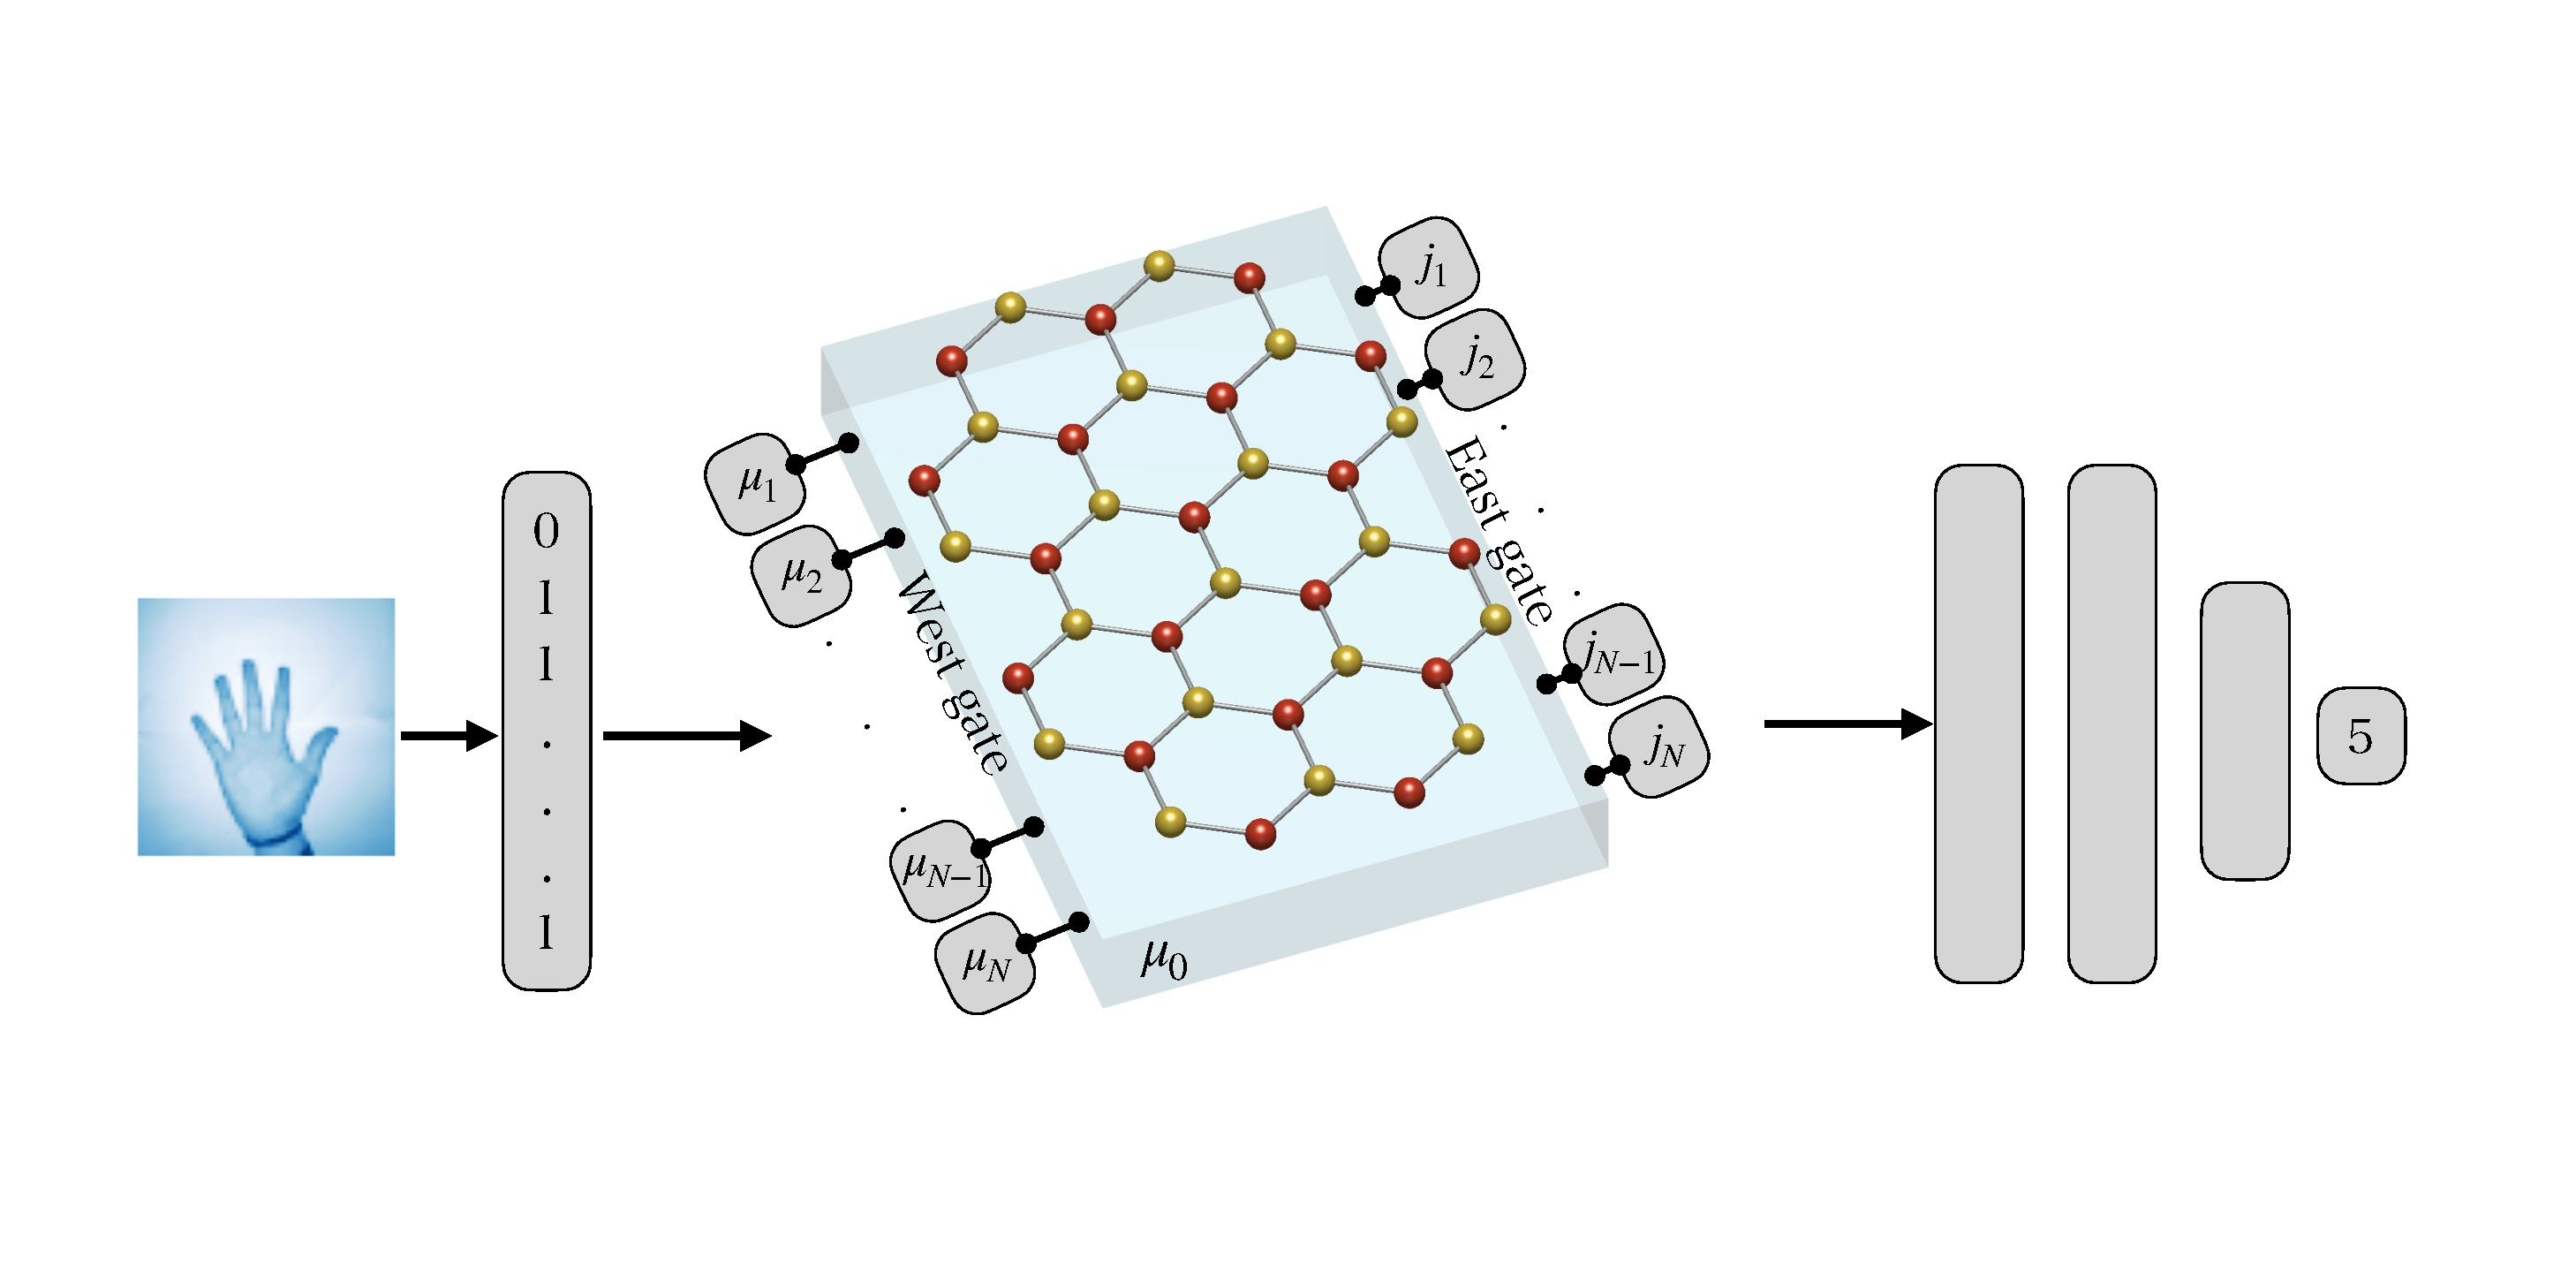
\includegraphics[width=0.8\linewidth]{Figures_for_notes/GrapheneNN.pdf}
        \caption{Proposed graphene-based neuromorphic network architecture.}
        \label{fig:grapheneNN}
    \end{figure}

    In physical neural hardware, the role of the first layers of a neural network can be assumed by an untrained, fixed physical system whose intrinsic linear and nonlinear responses generate high-dimensional feature maps. The computational cost associated with large matrix multiplications is effectively replaced by wave propagation or transport through the medium itself, with training relegated to a simple linear readout. This paradigm introduces novel performance and the energy-efficiency solid state alternatives to existent costly pre-instructed logic.

    Let us begin by clarifying which aspects of neural-network-style feature extraction can, and cannot, be implemented using a physical electronic system such as graphene. Naively, one would like to inject a signal into one side of the sample and interpret the scattered response—at the same or multiple frequencies—as a nonlinear feature representation of the input on the opposite side (see FIG.1). Now we acknowledge the constraints imposed by electrodynamics and transport and summarise options to consider:
    \begin{itemize}
        \item Inject current through specific terminals. Here we must be careful since the charge has also leave the sample ($I_L + I_R = 0$). This type is likely more dissipative. Injected AC current can be casted in the form of a vector potential, namely phase winding on one side of the system. Potentailly can be solved perturbatively?
        \item Apply a voltage between two contacts. Perhaps we can add a top and bottom contact and apply voltage left-top terminals and read out bot-right terminals. Here the issue is that we need to be very precise to state between what contacts voltage is applied.
    \end{itemize}

    Let's consider the voltage approach. We segment the West edge into N independently contacted reservoirs (labeled $i$). Each reservoir is biased by a voltage $V_i$ relative to a common ground (reference chemical potential $\mu_0$, which sets its electrochemical potential $\mu_i = \mu_0+ eV_i$. The binary input is encoded by choosing $V_i\in \{V_0, V_1\}$. The output segment is the East edge where we measure the currents  $j_i$.

    Additional points:
    \begin{itemize}
        \item For slow drives, we can do $V_i\rightarrow V_i(t)$ thus nonlinear responses of $j_i$.
        \item Graphene can be a subject to external radiation or a transverse voltage. Once strained - nonlinear effects.
    \end{itemize}

    Let's begin on solidification of the problem from defining the system Hamiltonian:
    \begin{equation}
    H_{\rm graphene}
    = -t\sum_{\langle r,r'\rangle\in C}\big(c_r^\dagger c_{r'} + \text{h.c.}\big)
     ,\qquad H_{\rm West~terminals} =\sum_{i=1}^N\left[\sum_{k_i} (\epsilon_{i {k_i}}-\mu_i) a_{i {k_i}}^\dagger a_{i {k_i}}\right], 
    \end{equation}

    Unlike West terminals, East are all at rest ($\mu_0$), so without applied voltage we are in the equilibrium:
    \begin{equation}
     H_{\rm East~terminals} =\sum_{i=1}^M\left[\sum_{k_i} (\epsilon_{i {k_i}}-\mu_0) b_{i{k_i}}^\dagger b_{i {k_i}}\right],  
    \end{equation}
    
    % ===== Coupling between lead alpha and boundary sites of graphene =====
    \begin{equation}
    H_{\rm tunneling~West}
    = \sum_{\alpha,k}\sum_{r\in\partial_W G}
    \left(V_{\alpha k,r}\, a_{\alpha k}^\dagger c_r + \text{h.c.}\right),\qquad H_{\rm tunneling~East}
    = \sum_{\alpha,k}\sum_{r\in\partial_E G}
    \left(V_{\alpha k,r}\, b_{\alpha k}^\dagger c_r + \text{h.c.}\right).
    \end{equation}
    
    The current at each east terminal is defined and the change change per time:
    \begin{equation}
    \hat I_j
    = -e\,\frac{d\hat N^E_j}{dt}
    = -\frac{ie}{\hbar}\,[H_{\rm tot},\hat N^E_j]
    = -\frac{ie}{\hbar}\sum_{k}\sum_{r\in{r_j}}
    \left(V_{\alpha k,r}\, b_{j k}^\dagger c_r
    - V_{\alpha k,r}^*\, c_r^\dagger b_{j k}\right).
    \end{equation}
    
    The tricky part is to find the expectation value for such currents, we will need to understand the DM of the system $j_\alpha = \langle \hat \rho \hat{I}_\alpha \rangle.$ If we proceed in the similar fashion as in the Josephson junction, we write the perturbation theory for $\rho$ is coupling to the leads, then the leading current component is $j_\alpha = \langle \hat \rho^{(1)} \hat{I}_\alpha \rangle.$ $ \rho^{(1)} =\hat{\rho}_{\rm graphene}\Pi\otimes_{\alpha\in\{W,E\}}\hat{\rho}_\alpha $ is simply direct product of subsystems. We will need some adiabaticity regularization statements + request large memory-less large reservoirs (leads). 

    \subsection{Numerical validation roadmap}

    Rather than pursuing a fully analytic evaluation of the multi-terminal mapping
    \(\{V_i\}\mapsto \{I_j\}\) for a finite graphene flake coupled to many reservoirs,
    we propose a two-tier numerical program that is standard in mesoscopic transport.
    
    \paragraph{Tier 1 (fast proof-of-principle): diffusive / resistor-network model.}
    We first construct a classical baseline in the diffusive limit by treating the graphene sheet
    as a two-dimensional conductor with (possibly inhomogeneous) conductivity \(\sigma(\mathbf r)\).
    The electrostatic potential \(\phi(\mathbf r)\) is obtained from the stationary conduction equation`
    \begin{equation}
    \nabla\!\cdot\!\big(\sigma(\mathbf r)\nabla \phi(\mathbf r)\big)=0,
    \qquad
    \mathbf j(\mathbf r)=-\sigma(\mathbf r)\nabla \phi(\mathbf r).
    \end{equation}
    The West edge is segmented into \(N\) independently biased contacts imposing boundary values
    \(\phi|_{W_i}=V_i\) (binary encoding \(V_i\in\{V_0,V_1\}\)), while the East edge is segmented into
    \(M\) drain contacts held at a reference potential (e.g. \(\phi|_{E_j}=0\)).
    The output features are the terminal currents
    \begin{equation}
    I_j = \int_{E_j} \mathbf j(\mathbf r)\cdot d\mathbf S,
    \qquad j=1,\dots,M,
    \end{equation}
    which define a high-dimensional feature map \(\{V_i\}\mapsto \{I_j\}\).
    This tier enables rapid scaling studies (large \(N,M\)), robustness to disorder in \(\sigma(\mathbf r)\),
    and geometry/contact-configuration sweeps at minimal computational cost.
    
    \paragraph{Tier 2 (physics-faithful): quantum-coherent tight-binding transport (Kwant).}
    We then validate the same architecture within a coherent tight-binding description of a finite graphene flake
    coupled to \(N+M\) leads, using the Landauer--B\"uttiker framework as implemented in the \texttt{kwant} library.
    The West input contacts are modeled as independent reservoirs with chemical potentials
    \(\mu_i=\mu_0+eV_i\), and the East drains are held at \(\mu_0\) (current readout), yielding terminal currents
    \begin{equation}
    I_\alpha
    = \frac{2e}{h}\sum_{\beta}\int dE\;
    T_{\alpha\beta}(E)\,\big[f_\beta(E)-f_\alpha(E)\big],
    \end{equation}
    with transmissions \(T_{\alpha\beta}(E)\) computed from the device Hamiltonian and lead self-energies.
    This tier quantifies the influence of quantum interference, mode structure, and backscattering on the
    feature map and allows controlled tests versus disorder strength, Fermi energy, and (optionally) magnetic field.
    
    \paragraph{Outcome.}
    Tier 1 establishes feasibility and scaling of the feature-generation concept in the diffusive limit,
    while Tier 2 provides a quantitative, community-standard transport validation in a microscopic graphene model.
    Together they provide a practical route to demonstrate \(\{V_i\}\mapsto\{I_j\}\) feature generation without
    requiring a fully analytic closed-form solution.

    Details \paragraph{Governing equations.}
    In the diffusive (ohmic) regime, the electrostatic potential $\phi(\mathbf r)$
    and current density $\mathbf j(\mathbf r)$ satisfy
    \begin{equation}
    \mathbf j(\mathbf r) = \sigma(\mathbf r)\,\mathbf E(\mathbf r)
    = -\,\sigma(\mathbf r)\,\nabla \phi(\mathbf r),
    \label{eq:ohm}
    \end{equation}
    together with steady-state charge conservation
    \begin{equation}
    \nabla\cdot \mathbf j(\mathbf r)=0.
    \label{eq:cont}
    \end{equation}
    Combining Eqs.~\eqref{eq:ohm}--\eqref{eq:cont} yields the elliptic PDE
    \begin{equation}
    \nabla\cdot\!\big(\sigma(\mathbf r)\,\nabla \phi(\mathbf r)\big)=0.
    \label{eq:pde}
    \end{equation}
    
    \paragraph{Boundary conditions.}
    On metallic contacts (Dirichlet boundaries) we fix the potential:
    \begin{equation}
    \phi|_{W_i}=V_i, \qquad i=1,\dots,N,
    \qquad\text{and}\qquad
    \phi|_{E_j}=0, \qquad j=1,\dots,M.
    \label{eq:dirichlet}
    \end{equation}
    On insulating boundaries (Neumann boundaries) we enforce zero normal current:
    \begin{equation}
    \mathbf n\cdot \mathbf j = -\,\mathbf n\cdot \sigma\nabla\phi = 0.
    \label{eq:neumann}
    \end{equation}
    
    \paragraph{Finite-volume discretization and linear system $A\phi=b$.}
    Discretize the domain on a rectangular grid with spacings $\Delta x,\Delta y$,
    and denote $\phi_{i,j}\equiv \phi(x_i,y_j)$.
    Define the face conductivities by arithmetic averaging,
    \begin{equation}
    \sigma_{i+\frac12,j}=\frac{\sigma_{i+1,j}+\sigma_{i,j}}{2},
    \qquad
    \sigma_{i,j+\frac12}=\frac{\sigma_{i,j+1}+\sigma_{i,j}}{2},
    \label{eq:sigfaces}
    \end{equation}
    (and analogously for $\sigma_{i-\frac12,j}$ and $\sigma_{i,j-\frac12}$).
    The fluxes through the four faces of the control volume around node $(i,j)$ are
    \begin{align}
    J_x^{+} &= -\,\sigma_{i+\frac12,j}\,\frac{\phi_{i+1,j}-\phi_{i,j}}{\Delta x},&
    J_x^{-} &= -\,\sigma_{i-\frac12,j}\,\frac{\phi_{i,j}-\phi_{i-1,j}}{\Delta x}, \\
    J_y^{+} &= -\,\sigma_{i,j+\frac12}\,\frac{\phi_{i,j+1}-\phi_{i,j}}{\Delta y},&
    J_y^{-} &= -\,\sigma_{i,j-\frac12}\,\frac{\phi_{i,j}-\phi_{i,j-1}}{\Delta y}.
    \label{eq:fluxes}
    \end{align}
    Steady-state conservation $\nabla\cdot \mathbf j=0$ becomes (discrete divergence)
    \begin{equation}
    \frac{J_x^{+}-J_x^{-}}{\Delta x}+\frac{J_y^{+}-J_y^{-}}{\Delta y}=0,
    \label{eq:discdiv}
    \end{equation}
    i.e.
    \begin{equation}
    \frac{\sigma_{i+\frac12,j}}{\Delta x^{2}}\!\left(\phi_{i+1,j}-\phi_{i,j}\right)
    -\frac{\sigma_{i-\frac12,j}}{\Delta x^{2}}\!\left(\phi_{i,j}-\phi_{i-1,j}\right)
    +\frac{\sigma_{i,j+\frac12}}{\Delta y^{2}}\!\left(\phi_{i,j+1}-\phi_{i,j}\right)
    -\frac{\sigma_{i,j-\frac12}}{\Delta y^{2}}\!\left(\phi_{i,j}-\phi_{i,j-1}\right)=0.
    \label{eq:stencil}
    \end{equation}
    Rearranging gives the linear five-point stencil
    \begin{align}
    \Bigg(
    \frac{\sigma_{i+\frac12,j}+\sigma_{i-\frac12,j}}{\Delta x^{2}}
    +
    \frac{\sigma_{i,j+\frac12}+\sigma_{i,j-\frac12}}{\Delta y^{2}}
    \Bigg)\phi_{i,j}
    &-\frac{\sigma_{i+\frac12,j}}{\Delta x^{2}}\,\phi_{i+1,j}
    -\frac{\sigma_{i-\frac12,j}}{\Delta x^{2}}\,\phi_{i-1,j}\nonumber\\
    &-\frac{\sigma_{i,j+\frac12}}{\Delta y^{2}}\,\phi_{i,j+1}
    -\frac{\sigma_{i,j-\frac12}}{\Delta y^{2}}\,\phi_{i,j-1}=0,
    \label{eq:row}
    \end{align}
    which provides one row of a sparse linear system $A\boldsymbol{\phi}=\mathbf b$.
    Dirichlet nodes are imposed by replacing the corresponding row with
    \begin{equation}
    \phi_{i,j}=V_{i,j}^{(\mathrm{dir})},
    \label{eq:dirrow}
    \end{equation}
    while any neighbor value fixed by Dirichlet conditions is moved to the right-hand side $\mathbf b$.

{\bf Short note} after discussion. We identified the main problems of flat bulk device (without some chiral channels): 

1.	Resistive bulk – diffusion quickly washes away information.

2.	Whether diffusion in resistive network could work as neural network operation?

3. \textcolor{blue}{How do people solve problem 2 above?} They solve it by encoding information via scatterers. Due to Born series, this creates linear + potential times nonlinearity output.

\section{Machine learning benchmarks of graphene optical filter}
\subsection{Digit mnist simple classifier}
In this section we discuss digit-MNIST dataset benchmarks. The main trick about this dataset is that people know very well how to achieve 99.5\%+ accuracy on that. So, our benchmark is done for relatively simple classifier, where the positive or negative change would be visible. We use the following idea: input $X$ is sued for regular classifier. Then, we use the fact that graphene could provide $X^2$ in another frequency, so we could compose twice bigger image of $\{X,X^2\}$. To avoid a problem of having more trainable parameters, we make convolutional layers larger, and dense trainable layers to be the same size. The structures are shown in Fig.\ref{fig:mnist-conv-classifiers-simple-schemes}.
\begin{figure}
    \centering
    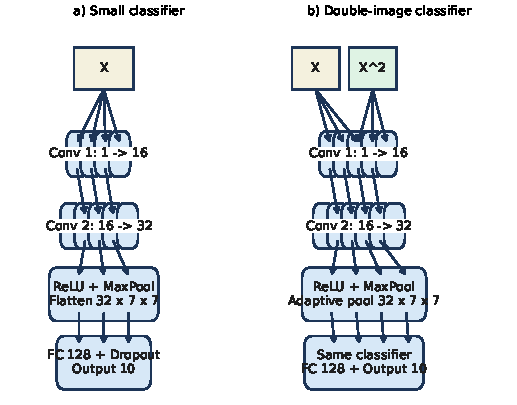
\includegraphics[scale=1.0]{Figures_for_notes/double_image_classifier_schemes.pdf}
    \caption{Schemes of MNIST classifiers used to test additional nonlinear output provided by graphene.}
    \label{fig:mnist-conv-classifiers-simple-schemes}
\end{figure}

The results of banchmarking are shown in Fig.\ref{fig:digit-mnist-benchmarking-small}.
\begin{figure}
    \centering
    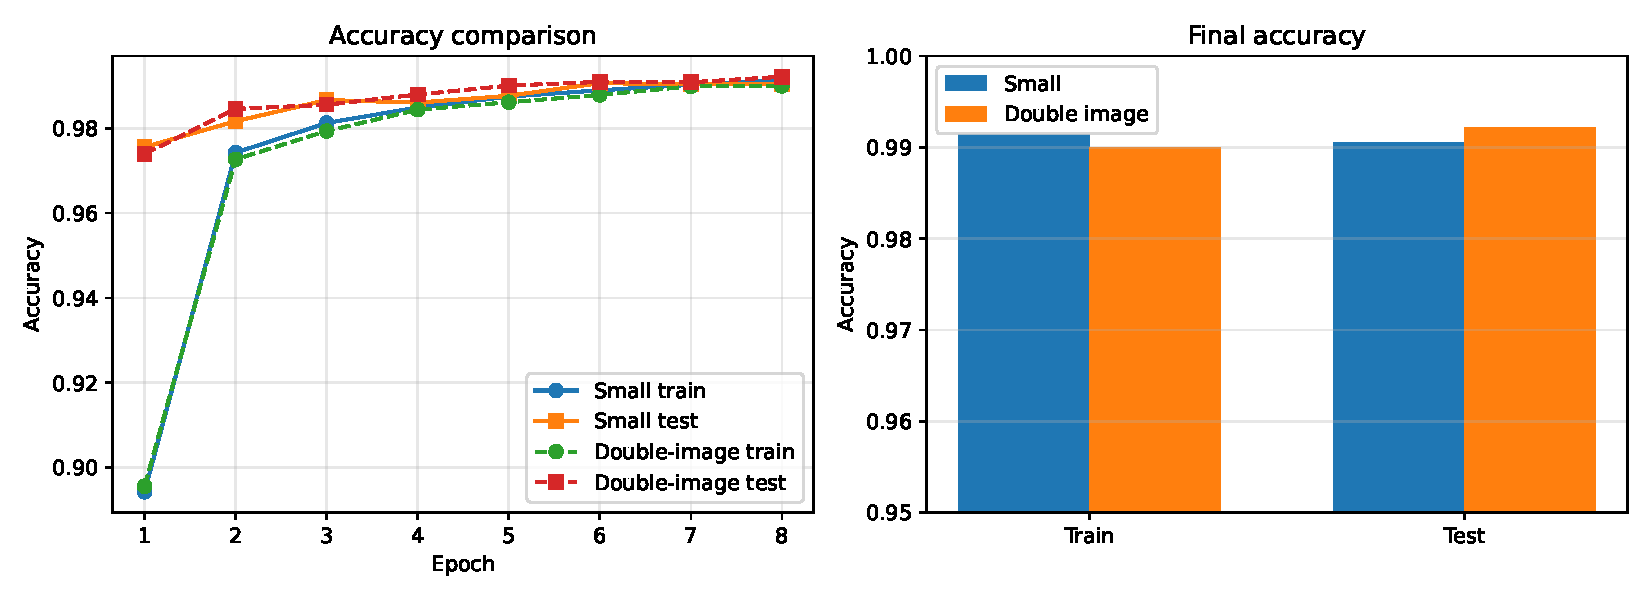
\includegraphics[scale=0.5]{Figures_for_notes/accuracy_comparison_mnist_digits_small_classifiers.pdf}
    \caption{Benchmarking of train and test accuracies of classifier applied to regular mnist, and to mnist with extra quadratic image together. Results: Small classifier      | train: 99.1350\% | test: 99.0500\%
Double-image classifier | train: 99.0017\% | test: 99.2200\%.}
    \label{fig:digit-mnist-benchmarking-small}
\end{figure}

\begin{figure}
    \centering
    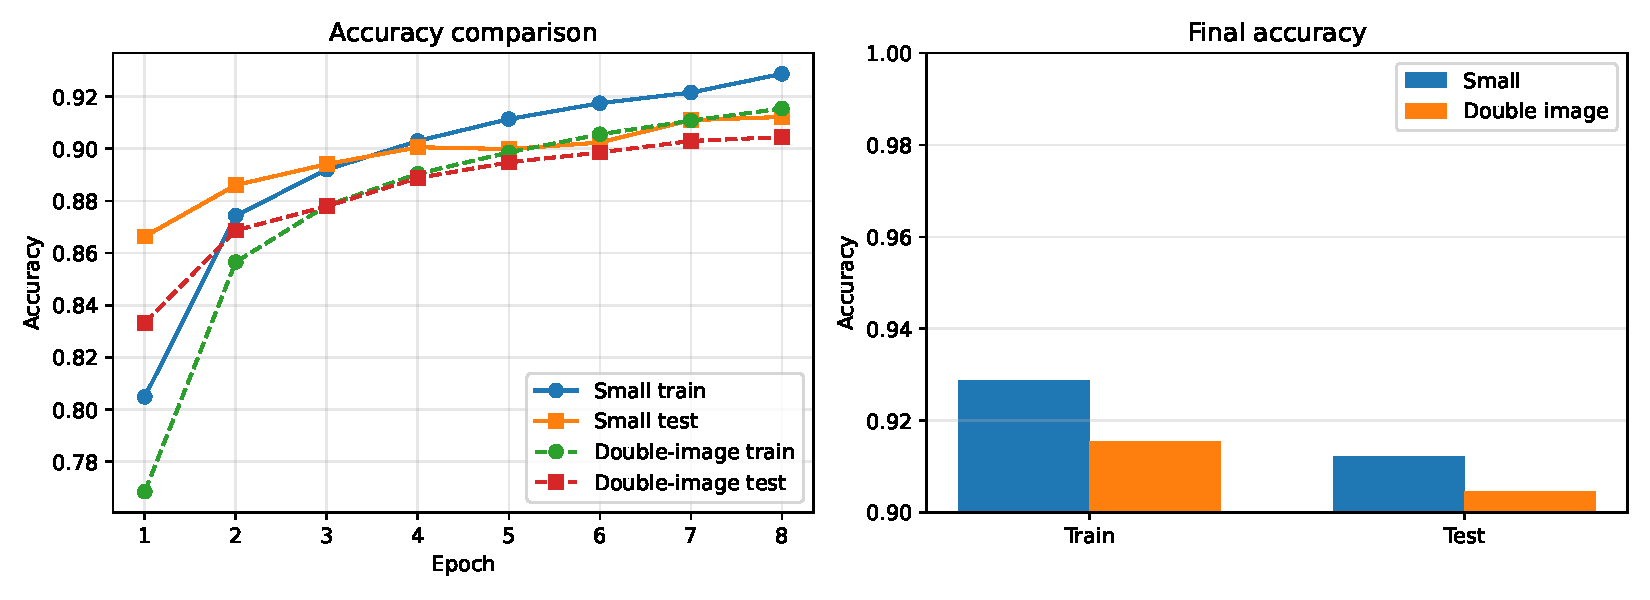
\includegraphics[scale=0.5]{Figures_for_notes/accuracy_comparison_fashion_mnist_digits_small_classifiers.pdf}
    \caption{Benchmarking of train and test accuracies of classifier applied to fashion-mnist, and to fashion-mnist with extra quadratic image together. Results: Small classifier      | train: 92.8717\% | test: 91.2200\%
Double-image classifier | train: 91.5450\% | test: 90.4500\%.}
    \label{fig:fashion-mnist-benchmarking-small}
\end{figure}

\bibliography{neuromorph_graphene_bib} 
\end{document}
On side 1,
\begin{align}
\mathbf{E}^1 &= e^{i(kz - \omega t)} \mathbf{E}^i + e^{i(-kz - \omega t)} \mathbf{E}^r 
= e^{i(kz - \omega t)} \begin{pmatrix} E_x^i \\ E_y^i \end{pmatrix} 
+ e^{i(-kz - \omega t)} \begin{pmatrix} E_x^r \\ E_y^r \end{pmatrix},  \label{side1Eq1}\\
\mathbf{H}^1 &= e^{i(kz - \omega t)} \mathbf{H}^i + e^{i(-kz - \omega t)} \mathbf{H}^r 
= e^{i(kz - \omega t)} \begin{pmatrix} H_x^i \\ H_y^i \end{pmatrix} 
+ e^{i(-kz - \omega t)} \begin{pmatrix} H_x^r \\ H_y^r \end{pmatrix}.\label{side1Eq2}
\end{align}

On side 2,
\begin{align}
\mathbf{E}^2 &= e^{i(kz - \omega t)} \mathbf{E}^t 
= e^{i(kz - \omega t)} \begin{pmatrix} E_x^t \\ E_y^t \end{pmatrix},\label{side2Eq1} \\
\mathbf{H}^2 &= e^{i(kz - \omega t)} \mathbf{H}^t 
= e^{i(kz - \omega t)} \begin{pmatrix} H_x^t \\ H_y^t \end{pmatrix}.\label{side2Eq2}
\end{align}

Let us also assume that the current is only on the 2D interface and that the current-less space is homogeneous. The Maxwell equations in the current-less space read:
\begin{equation}
\nabla \times \mathbf{E} = - \frac{\partial \mathbf{B}}{\partial t} = -\mu \frac{\partial \mathbf{H}}{\partial t}, \qquad
\nabla \times \mathbf{H} = \frac{\partial \mathbf{D}}{\partial t} = \epsilon \frac{\partial \mathbf{E}}{\partial t}. 
\end{equation}

THe above can be rewritten as:
\begin{align}
\frac{\partial}{\partial z} E_x &= - \mu \frac{\partial}{\partial t} H_y, \qquad
\frac{\partial}{\partial z} E_y = \mu \frac{\partial}{\partial t} H_x, \\
\frac{\partial}{\partial z} H_x &= \epsilon \frac{\partial}{\partial t} E_y, \qquad
\frac{\partial}{\partial z} H_y = - \epsilon \frac{\partial}{\partial t} E_x. 
\end{align}

from comparing the plane wave factors in Eq.~\eqref{side1Eq1}-Eq.\eqref{side1Eq2}, we conclude:
\begin{align*}
ik E_x^i &= i \omega \mu H_y^i, \qquad
ik E_y^i = -i \omega \mu H_x^i, \qquad
ik H_x^i = -i \omega \epsilon E_y^i, \qquad
ik H_y^i = i \omega \epsilon E_x^i, \\
-ik E_x^r &= i \omega \mu H_y^r, \qquad
-ik E_y^r = -i \omega \mu H_x^r, \qquad
-ik H_x^r = -i \omega \epsilon E_y^r, \qquad
-ik H_y^r = i \omega \epsilon E_x^r,
\end{align*}

and Eq.~\eqref{side2Eq1}-Eq.\eqref{side2Eq2}
\begin{align*}
ik E_x^t &= i \omega \mu H_y^t, \qquad
ik E_y^t = -i \omega \mu H_x^t, \qquad
ik H_x^t = -i \omega \epsilon E_y^t, \qquad
ik H_y^t = i \omega \epsilon E_x^t.
\end{align*}

Namely,
\begin{align}
H_y^i &= \sqrt{\frac{\epsilon}{\mu}}\, E_x^i, \qquad
H_x^i = -\sqrt{\frac{\epsilon}{\mu}}\, E_y^i, \qquad
H_y^r = \sqrt{\frac{\epsilon}{\mu}}\, E_x^r, \\
H_x^r &= \sqrt{\frac{\epsilon}{\mu}}\, E_y^r, \qquad
H_y^t = \sqrt{\frac{\epsilon}{\mu}}\, E_x^t, \qquad
H_x^t = -\sqrt{\frac{\epsilon}{\mu}}\, E_y^t,
\end{align} 

where we have utilized
\begin{equation}
\frac{k}{\omega \mu} = \frac{1}{v \mu} = \frac{\sqrt{\mu \epsilon}}{\mu} = \sqrt{\frac{\epsilon}{\mu}} = c\epsilon_0.
\end{equation}

Therefore we can write Eqs.~(\ref{side1Eq1}-\ref{side1Eq2}) as
\begin{align}
\mathbf{E}^1 &= e^{i(kz - \omega t)} \mathbf{E}^i + e^{i(-kz - \omega t)} \mathbf{E}^r
= e^{i(kz - \omega t)} \begin{pmatrix} E_x^i \\ E_y^i \end{pmatrix} 
+ e^{i(-kz - \omega t)} \begin{pmatrix} E_x^r \\ E_y^r \end{pmatrix}, \nonumber \\
\mathbf{H}^1 &= e^{i(kz - \omega t)} \mathbf{H}^i + e^{i(-kz - \omega t)} \mathbf{H}^r \nonumber \\
&= \sqrt{\frac{\epsilon}{\mu}} \left[ e^{i(kz - \omega t)} \begin{pmatrix} -E_y^i \\ E_x^i \end{pmatrix} 
+ e^{i(-kz - \omega t)} \begin{pmatrix} E_y^r \\ -E_x^r \end{pmatrix} \right],
\end{align}

\begin{align}
\mathbf{E}^2 &= e^{i(kz - \omega t)} \mathbf{E}^t
= e^{i(kz - \omega t)} \begin{pmatrix} E_x^t \\ E_y^t \end{pmatrix}, \nonumber \\
\mathbf{H}^2 &= e^{i(kz - \omega t)} \mathbf{H}^t
= \sqrt{\frac{\epsilon}{\mu}}\, e^{i(kz - \omega t)} \begin{pmatrix} -E_y^t \\ E_x^t \end{pmatrix}.
\end{align}

According to the boundary conditions for electromagnetic fields, on the interface between medium 1 and 2, the tangential component of the electric field is continuous, and
\begin{equation}
\mathbf{n}_{12} \times \left( \mathbf{E}^2 - \mathbf{E}^1 \right) = \boldsymbol{\alpha},\qquad \mathbf{n}_{12} \times \left( \mathbf{H}^2 - \mathbf{H}^1 \right) = \boldsymbol{\alpha}.
\end{equation}
where $\boldsymbol{\alpha}$ is the current density on the interface. Notice this is the \textbf{single} place where medium contributes! We take $\mathbf{n}_{12} = \hat{\mathbf{z}}$. For the electric field, we find:
\begin{align}
E_x^t - \left( E_x^i + E_x^r \right) &= 0,\label{14} \\
E_y^t - \left( E_y^i + E_y^r \right) &= 0,\label{15}
\end{align}
while for magnetic
\begin{align}
H_x^2 - H_x^1 &= j_y, \\
H_y^2 - H_y^1 &= - j_x.
\end{align}
which equivalently, assuming that both mediums being vacuums, becomes:
\begin{align}
- c \epsilon_0 E_y^t - c \epsilon_0 \left( - E_y^i + E_y^r \right) &= j_y 
= \sigma_{yx} E_x^t + \sigma_{yy} E_y^t, \label{16} \\
c \epsilon_0 E_x^t - c \epsilon_0 \left( E_x^i - E_x^r \right) &= - j_x 
= - \left( \sigma_{xx} E_x^t + \sigma_{xy} E_y^t \right),\label{17}
\end{align}


Now we let \textit{Mathematica} solve Eqs.~(\ref{14},\ref{15},\ref{16},\ref{17}), we would have 
\begin{align}
E_x^r &= -\frac{2c E_x^i \epsilon_0 \sigma_{xx} + 2c E_y^i \epsilon_0 \sigma_{xy} - E_x^i \sigma_{xy} \sigma_{yx} + E_x^i \sigma_{xx} \sigma_{yy}}
{4c^2 \epsilon_0^2 + 2c \epsilon_0 \sigma_{xx} - \sigma_{xy} \sigma_{yx} + 2c \epsilon_0 \sigma_{yy} + \sigma_{xx} \sigma_{yy}},\label{s1} \\
E_y^r &= -\frac{-2c E_x^i \epsilon_0 \sigma_{yx} + E_y^i \sigma_{xy} \sigma_{yx} - 2c E_y^i \epsilon_0 \sigma_{yy} - E_y^i \sigma_{xx} \sigma_{yy}}
{-4c^2 \epsilon_0^2 - 2c \epsilon_0 \sigma_{xx} + \sigma_{xy} \sigma_{yx} - 2c \epsilon_0 \sigma_{yy} - \sigma_{xx} \sigma_{yy}}, \\
E_x^t &= \frac{2 \left( 2c^2 E_x^i \epsilon_0^2 - c E_y^i \epsilon_0 \sigma_{xy} + c E_x^i \epsilon_0 \sigma_{yy} \right)}
{4c^2 \epsilon_0^2 + 2c \epsilon_0 \sigma_{xx} - \sigma_{xy} \sigma_{yx} + 2c \epsilon_0 \sigma_{yy} + \sigma_{xx} \sigma_{yy}}, \\
E_y^t &= -\frac{2 \left( -2c^2 E_y^i \epsilon_0^2 - c E_y^i \epsilon_0 \sigma_{xx} + c E_x^i \epsilon_0 \sigma_{yx} \right)}
{4c^2 \epsilon_0^2 + 2c \epsilon_0 \sigma_{xx} - \sigma_{xy} \sigma_{yx} + 2c \epsilon_0 \sigma_{yy} + \sigma_{xx} \sigma_{yy}}.\label{s2}
\end{align}

The polarization of the transmitted and the reflected light can then be obtained with this.
\newpage
\subsubsection{Reflection matrix}
The reflection matrix is defined as:
\begin{equation}
    \mathbf{E}^r = \left(\begin{array}{cc}
        r_{xx} & r_{xy} \\
        -r_{yx} & r_{yy} 
    \end{array}\right)\mathbf{E}^i.
\end{equation}
Notice denominators in Eqs.(\ref{s1}-\ref{s2}) will not matter, we will label those by D. For isotropic system we find
\begin{align}
    E_x^r &= -\frac{2c E_x^i \epsilon_0 \sigma_{xx} + 2c E_y^i \epsilon_0 \sigma_{xy} - E_x^i \sigma_{xy} \sigma_{yx} + E_x^i \sigma^2_{xx} }
{4c^2 \epsilon_0^2 + 2c \epsilon_0 \sigma_{xx} - \sigma_{xy} \sigma_{yx} + 2c \epsilon_0 \sigma_{yy} + \sigma_{xx} \sigma_{yy}}, \\
E_y^r &= -\frac{2c E_x^i \epsilon_0 \sigma_{yx} - E_y^i \sigma_{xy} \sigma_{yx} + 2c E_y^i \epsilon_0 \sigma_{yy} + E_y^i \sigma^2_{xx} }
{4c^2 \epsilon_0^2 + 2c \epsilon_0 \sigma_{xx} - \sigma_{xy} \sigma_{yx} + 2c \epsilon_0 \sigma_{yy} + \sigma_{xx} \sigma_{yy}},
\end{align}
now, we write:
\begin{equation}
    \frac{r_{xy}D}{(c\epsilon_0)^2} = - 2\tilde\sigma_{xy},\qquad \frac{r_{xx}D}{c  \epsilon_0} = -2\tilde\sigma_{xx} - \tilde\sigma^2_{xy}  -  \tilde\sigma^2_{xx}
\end{equation}
where $\tilde \sigma = \sigma/(c\epsilon_0),$ that we use to find the Kerr angle:
\begin{equation}
    \theta_K = -\frac{1}{2}({\rm arg}[ r_+] - {\rm arg} [r_-]), \quad \text{for} \quad r_{\pm} = r_{xx} \mp i r_{xy}
\end{equation}
For superconducting system (Oles will fix next Eqs soon):
\begin{equation}
    [\tilde\sigma^{(1)}]^{xx}_\omega=- i\frac{e^2}{\hbar c\epsilon_0}\frac{1}{\hbar\omega}\sum_a f_a\partial^x h^x_{aa}, \qquad  [\tilde\sigma^{(1)}]^{xy}_\omega=- i\frac{e^2}{\hbar c\epsilon_0}\sum_{ab}\frac{h^x_{ab}h^y_{ba}f_{ab}}{\hbar\omega -\mathcal{E}_{ab}+ i\eta}\frac{1}{\mathcal{E}_{ba}},
\end{equation}
so we need to compute it for somewhat nonzero $\omega$ to get anything. $\tilde\sigma_{xx}=\alpha\rho/\hbar\omega=-50meV/\hbar\omega$, so we can write for $\alpha = \frac{e^2}{\hbar c\epsilon_0}$:
\begin{equation}
    r_\pm = -i\frac{\alpha^2\rho^2}{(\hbar \omega)^2}\mp\alpha\sum_{ab}\frac{h^x_{ab}h^y_{ba}f_{ab}}{\hbar\omega -\mathcal{E}_{ab}+ i\eta}\frac{1}{\mathcal{E}_{ba}}
\end{equation}

thus
\begin{equation}
    \theta_K = {\rm arctan}\left[\frac{(\hbar \omega)^2}{\alpha\rho^2}\sum_{ab}\frac{h^x_{ab}h^y_{ba}f_{ab}}{\hbar\omega -\mathcal{E}_{ab}+ i\eta}\frac{1}{\mathcal{E}_{ba}}\right]\approx \frac{(\hbar \omega)^2}{\alpha\rho^2}\sum_{ab}\frac{h^x_{ab}h^y_{ba}f_{ab}}{\hbar\omega -\mathcal{E}_{ab}+ i\eta}\frac{1}{\mathcal{E}_{ba}}
\end{equation}

I assumed $q_x= 10 \cdot 10^{-4}A^{-1}$, $\omega = 0.1$ meV $\theta_k = 5\cdot10^{-11}$.
\newpage
\section{Floquet Generalization to a nonlinear Kerr and Faraday effect}
Consider a Floquet convention:
\begin{equation}
    f(\omega) = \int dt f(t) e ^{i\omega t}, \qquad f(t) = \int \frac{d\omega}{2\pi}e^{-i\omega t}f(\omega),\qquad f(t)=f(t+T)=\sum_n f_ne^{-i\omega_n t}.
\end{equation}


On side 1,
\begin{align}
\mathbf{E}^1 &= e^{i(k_0z - \omega_0 t)} \mathbf{E}^i + \sum_{n} e^{i(-k_nz - \omega_n t)} \mathbf{E}^r_n 
= e^{i(k_0z - \omega_0 t)} \begin{pmatrix} E_x^i \\ E_y^i \end{pmatrix} 
+ \sum_ne^{i(-k_nz - \omega_n t)} \begin{pmatrix} E_{n,x}^r \\ E_{n,y}^r \end{pmatrix},  \label{Gside1Eq1}\\
\mathbf{H}^1 &= e^{i(k_0z - \omega_0 t)} \mathbf{H}^i + \sum_n e^{i(-k_nz - \omega_n t)} \mathbf{H}_n^r 
= e^{i(k_0z - \omega_0 t)} \begin{pmatrix} H_x^i \\ H_y^i \end{pmatrix} 
+ \sum_n e^{i(-k_nz - \omega_n t)} \begin{pmatrix} H_{n,x}^r \\ H_{n,y}^r \end{pmatrix}.\label{Gside1Eq2}
\end{align}

On side 2,
\begin{align}
\mathbf{E}^2 &= \sum_n e^{i(k_0z - \omega_n t)} \mathbf{E}_n^t 
= \sum_ne^{i(k_nz - \omega_n t)} \begin{pmatrix} E_{n,x}^t \\ E_{n,y}^t \end{pmatrix},\label{Gside2Eq1} \\
\mathbf{H}^2 &= \sum_n e^{i(k_0z - \omega_n t)} \mathbf{H}_n^t 
= \sum_n e^{i(k_nz - \omega_n t)} \begin{pmatrix} H_{n,x}^t \\ H_{n,y}^t \end{pmatrix}.\label{Gside2Eq2}
\end{align}
with $\omega_n = n\omega_0$

Let us also assume that the current is only on the 2D interface and that the current-less space is homogeneous. The Maxwell equations in the current-less space read:
\begin{equation}
\nabla \times \mathbf{E} = - \frac{\partial \mathbf{B}}{\partial t} = -\mu \frac{\partial \mathbf{H}}{\partial t}, \qquad
\nabla \times \mathbf{H} = \frac{\partial \mathbf{D}}{\partial t} = \epsilon \frac{\partial \mathbf{E}}{\partial t}. 
\end{equation}

The above can be rewritten as:
\begin{align}
\frac{\partial}{\partial z} E_x &= - \mu \frac{\partial}{\partial t} H_y, \qquad
\frac{\partial}{\partial z} E_y = \mu \frac{\partial}{\partial t} H_x, \\
\frac{\partial}{\partial z} H_x &= \epsilon \frac{\partial}{\partial t} E_y, \qquad
\frac{\partial}{\partial z} H_y = - \epsilon \frac{\partial}{\partial t} E_x. 
\end{align}

Thus in the media 1:
\begin{align}
\partial_z[e^{i(k_0z - \omega_0 t)}  E_x^i  
+ \sum_ne^{i(-k_nz - \omega_n t)}  E_{n,x}^r ] = -\mu \partial_t[e^{i(k_0z - \omega_0 t)}   H_y^i  
+ \sum_n e^{i(-k_nz - \omega_n t)} H_{n,y}^r]
\end{align}

\begin{align}
 \partial_z[e^{i(k_0z - \omega_0 t)} E_y^i  
+ \sum_ne^{i(-k_nz - \omega_n t)}  E_{n,y}^r ] = \mu \partial_t[e^{i(k_0z - \omega_0 t)} H_x^i  
+ \sum_n e^{i(-k_nz - \omega_n t)}H_{n,x}^r  ],
\end{align}
\begin{equation}
    \partial_z[e^{i(k_0z - \omega_0 t)} H_x^i  
+ \sum_n e^{i(-k_nz - \omega_n t)}H_{n,x}^r  ] = \epsilon \partial_t [e^{i(k_0z - \omega_0 t)} E_y^i  
+ \sum_ne^{i(-k_nz - \omega_n t)}  E_{n,y}^r ]
\end{equation}
\begin{equation}
    \partial_z[e^{i(k_0z - \omega_0 t)}   H_y^i  
+ \sum_n e^{i(-k_nz - \omega_n t)} H_{n,y}^r] = -\epsilon \partial_t[e^{i(k_0z - \omega_0 t)}  E_x^i  
+ \sum_ne^{i(-k_nz - \omega_n t)}  E_{n,x}^r]
\end{equation}
from comparing the plane wave factors, we conclude:
\begin{gather}
ik_0 E_x^i = i \omega_0 \mu H_y^i, \qquad
ik_0 E_y^i = -i \omega_0 \mu H_x^i, \qquad
ik_0 H_x^i = -i \omega_0 \epsilon E_y^i, \qquad
ik_0 H_y^i = i \omega_0 \epsilon E_x^i, \\
-ik_n E_{n,x}^r = i \omega_n \mu H_{n,y}^r, \qquad
-ik_n E_{n,y}^r = -i \omega_n \mu H_{n,x}^r, \qquad
-ik_n H_{n,x}^r = -i \omega_n \epsilon E_{n,y}^r, \qquad
-ik_n H_{n,y}^r = i \omega_n \epsilon E_{n,x}^r,
\end{gather}

and in the media 2:
Thus in the media 1:
\begin{align}
\partial_z[ \sum_ne^{i(k_nz - \omega_n t)}  E_{n,x}^t ] = -\mu \partial_t[\sum_n e^{i(k_nz - \omega_n t)} H_{n,y}^t]
\end{align}

\begin{align}
 \partial_z[\sum_ne^{i(k_nz - \omega_n t)}  E_{n,y}^t ] = \mu \partial_t[\sum_n e^{i(k_nz - \omega_n t)}H_{n,x}^t  ],
\end{align}
\begin{equation}
    \partial_z[\sum_n e^{i(k_nz - \omega_n t)}H_{n,x}^t  ] = \epsilon \partial_t [ \sum_ne^{i(k_nz - \omega_n t)}  E_{n,y}^t ]
\end{equation}
\begin{equation}
    \partial_z[\sum_n e^{i(k_nz - \omega_n t)} H_{n,y}^t] = -\epsilon \partial_t[\sum_ne^{i(k_nz - \omega_n t)}  E_{n,x}^t]
\end{equation}
with
\begin{align*}
ik_n E_{n,x}^t &= i \omega_n \mu H_{n,y}^t, \qquad
ik_n E_{n,y}^t = -i \omega_n \mu H_{n,x}^t, \qquad
ik_n H_{n,x}^t = -i\omega_n \epsilon E_{n,y}^t, \qquad
ik_n H_{n,y}^t = i \omega_n \epsilon E_{n,x}^t.
\end{align*}
Namely,
\begin{align}
H_y^i &= \sqrt{\frac{\epsilon}{\mu}}\, E_x^i, \qquad
H_x^i = -\sqrt{\frac{\epsilon}{\mu}}\, E_y^i, \qquad
H_{n,y}^r = \sqrt{\frac{\epsilon}{\mu}}\, E_{n,x}^r, \\
H_{n,x}^r &= \sqrt{\frac{\epsilon}{\mu}}\, E_{n,y}^r, \qquad
H_{n,y}^t = \sqrt{\frac{\epsilon}{\mu}}\, E_{n,x}^t, \qquad
H_{n,x}^t = -\sqrt{\frac{\epsilon}{\mu}}\, E_{n,y}^t,
\end{align} 

where we have utilized ($\omega_0 \equiv \omega$)
\begin{equation}
\frac{k_n}{\omega_n \mu} = \sqrt{\frac{\epsilon}{\mu}} 
\end{equation}


Therefore we can write
\begin{align}
\mathbf{E}^1 &
= e^{i(k_0z - \omega_0 t)} \begin{pmatrix} E_x^i \\ E_y^i \end{pmatrix} 
+\sum_{n\neq0} e^{i(-k_nz - \omega_n t)} \begin{pmatrix} E_{n,x}^r \\ E_{n,y}^r \end{pmatrix}, \nonumber \\
\mathbf{H}^1 &=  \sqrt{\frac{\epsilon}{\mu}} \left[ e^{i(kz -  \omega t)} \begin{pmatrix} -E_y^i \\ E_x^i \end{pmatrix} 
+ \sum_{n\neq0}e^{i(-k_nz - \omega_n t)} \begin{pmatrix}  E_{n,y}^r \\ - E_{n,x}^r \end{pmatrix} \right],
\end{align}

\begin{align}
\mathbf{E}^2 &= \sum_{n\neq0}e^{i(k_nz - \omega_n t)} \begin{pmatrix} E_{n,x}^t \\ E_{n,y}^t \end{pmatrix}, \nonumber \\
\mathbf{H}^2 &=\sqrt{\frac{\epsilon}{\mu}}\,\sum_{n\neq0} e^{i(k_nz - \omega_n t)} \begin{pmatrix} -E_{n,y}^t \\ E_{n,x}^t \end{pmatrix}.
\end{align}

According to the boundary conditions for electromagnetic fields, on the interface between medium 1 and 2, the tangential component of the electric field is continuous, and
\begin{equation}
\mathbf{n}_{12} \times \left( \mathbf{E}^2 - \mathbf{E}^1 \right) = 0,\qquad \mathbf{n}_{12} \times \left( \mathbf{H}^2 - \mathbf{H}^1 \right) = \boldsymbol{\alpha}.
\end{equation}
where $\boldsymbol{\alpha}$ is the current density on the interface. Notice this is the \textbf{single} place where medium contributes! We take $\mathbf{n}_{12} = \hat{\mathbf{z}}$. For the electric field, we find:
\begin{align}
E_x^t - \left( E_x^i + E_x^r \right) &= 0,\label{14} \\
E_y^t - \left( E_y^i + E_y^r \right) &= 0,\label{15}
\end{align}
while for magnetic
\begin{align}
H_x^2 - H_x^1 &= j_y, \\
H_y^2 - H_y^1 &= - j_x.
\end{align}
which equivalently, assuming that both mediums being vacuums, becomes for $n = 1$:
\begin{align}
- c \epsilon_0 E_{1,y}^t - c \epsilon_0 \left( - \delta_{n1}E_y^i + E_{1,y}^r \right) &= j_y 
= \sigma_{yx} E_{1,x}^t + \sigma_{yy} E_{n,y}^t,  \\
c \epsilon_0 E_{1, x}^t - c \epsilon_0 \left( \delta_{n1}E_{x}^i - E_{1,x}^r \right) &= - j_x 
= - \left( \sigma_{xx} E_{1,x}^t + \sigma_{xy} E_{1,y}^t \right),
\end{align}